\documentclass[a4j,11pt,twoside]{jbook}
\usepackage{ascmac}
\usepackage{amsmath}
\usepackage[dvipdfmx]{graphicx}
\usepackage{matx}
\usepackage{manyfloat}
\usepackage{caption}
\usepackage{geometry}
\usepackage{listings,jlisting}
\usepackage{listings}
\usepackage{color}
\captionsetup{labelformat=empty,labelsep=none}
\geometry{left=25mm,right=25mm,top=28mm,bottom=25mm}

\lstset{
	language=C,
	showstringspaces=f
	basicstyle={\ttfamily\small},
	tabsize=3,
	frame=trBL,
	numbers=left,
	numberstyle={\ttfamily\small},
	breaklines=true,
	backgroundcolor={\color[gray]{.96}},
}

\begin{document}

% --- title page --- %
\title{倒立振子の安定化制御}
\author{前田 拓}
\date{2017年7月12日}
\maketitle

% --- index --- %
\pagenumbering{roman}
\tableofcontents
\listoffigures
\listoftables
\pagenumbering{arabic}

% --- main --- %

% ----- chapter 1 ----- %
% ================================= chapter 1 ================================= %
\chapter{はじめに}
\section{目的}
本実験の目的は,倒立振子系を状態空間表現を用いて安定化制御し,線形不変システムを設計することである.
具体的に,次のことを目的とする.

\begin{itemize}
    \renewcommand{\labelenumi}{(\roman{enumi})}
    \item 倒立振子が安定化制御を行っている状態において,外乱による影響で振子が傾いたとき,倒立状態に戻すことができる (不安定平衡点の安定化).
    \item 倒立振子系に一定周期のパルス入力を与え,台車を目的の変位へ移動させる.
    \item 倒立振子が入力なしで静止している状態から,台車を動かすことにより振子を振り上げ,倒立状態にする (振り上げ制御).
\end{itemize}

\section{実験装置}

\begin{figure}[htbp]
    \begin{center}
        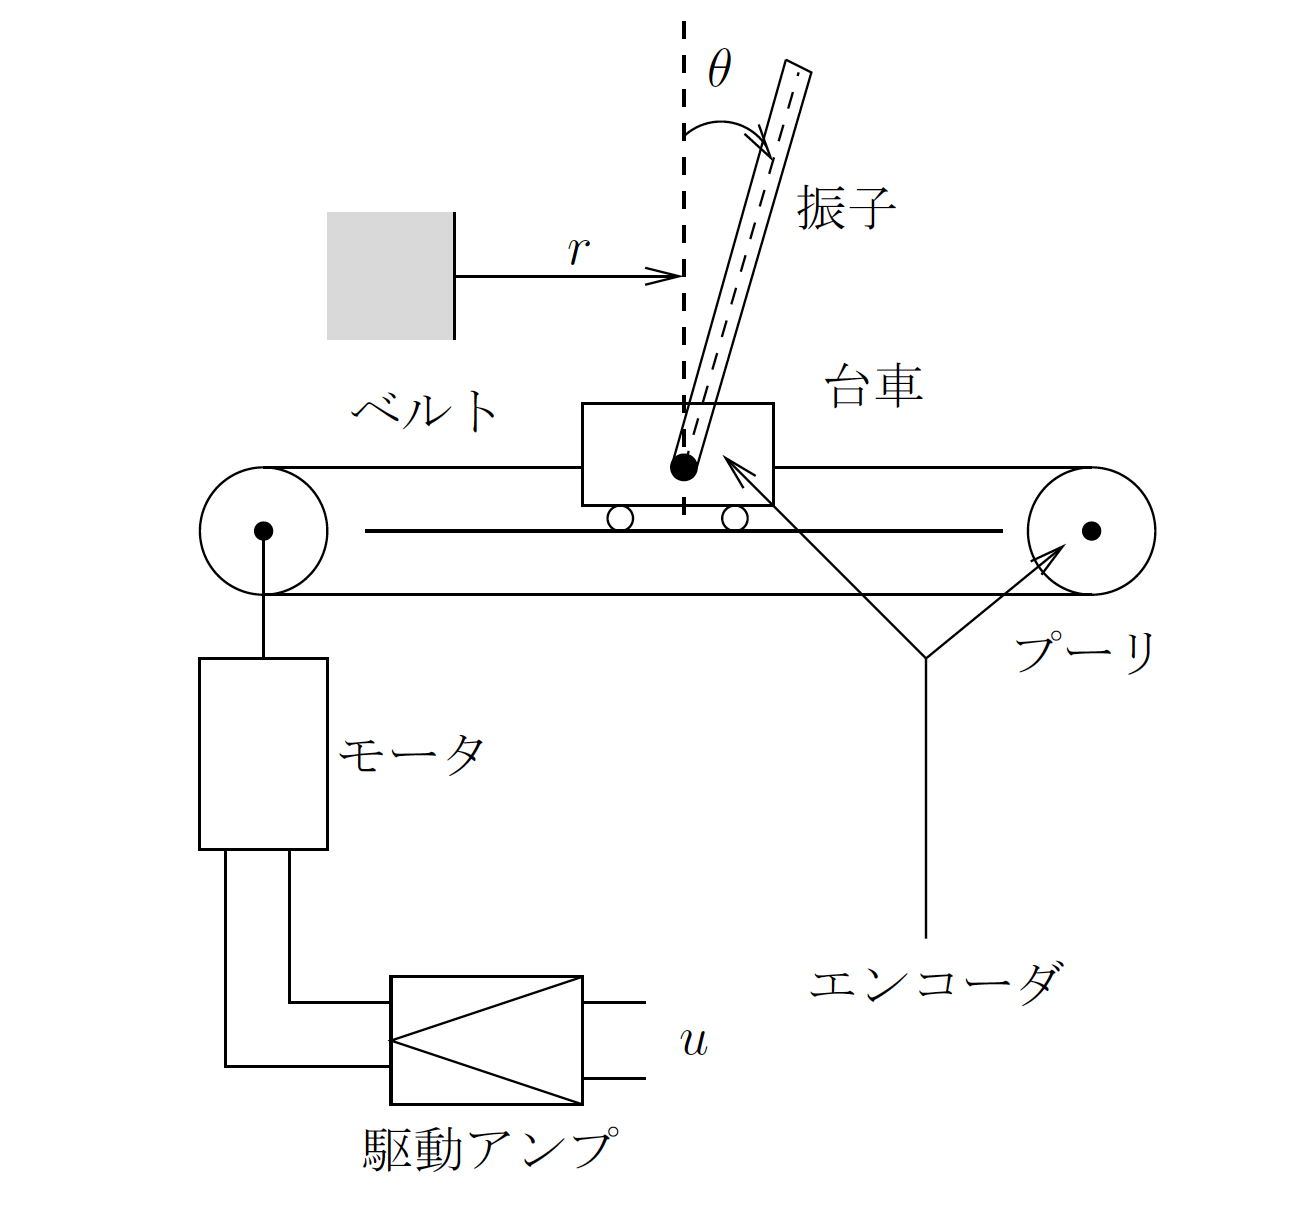
\includegraphics[width=0.6\linewidth]{model.png}
        \caption{図\ref{pendulum}: 倒立振子系}
        \label{pendulum}
    \end{center}
\end{figure}

図\ref{pendulum}は本実験で使用する倒立振子系である.
系は,モータ,ベルト,プーリ系から成り,台車はモータからの入力によりベルト上を水平方向に動くことができる.
台車の初期状態からの変位を$r$とする.
また,鉛直方向上向きから時計回りを正の方向として,台車に取り付けられた振子が回転した角度を$\theta$とする.
ポテンショメータにより,$r$と$\theta$を測定し,入力$u$を与える.

% =============================== chapter 1 END =============================== %

% --- Chapter 1 END --- %

% ----- chapter 2 ----- %
% ================================= chapter 2 ================================= %
\chapter{モデリング}
\label{chapter_modeling}
\section{数式モデル}
制御器の設計のため,倒立振子系の状態方程式,観測方程式から数式モデルを導出する.

\subsection{状態方程式}

\begin{figure}[htbp]
    \begin{center}
        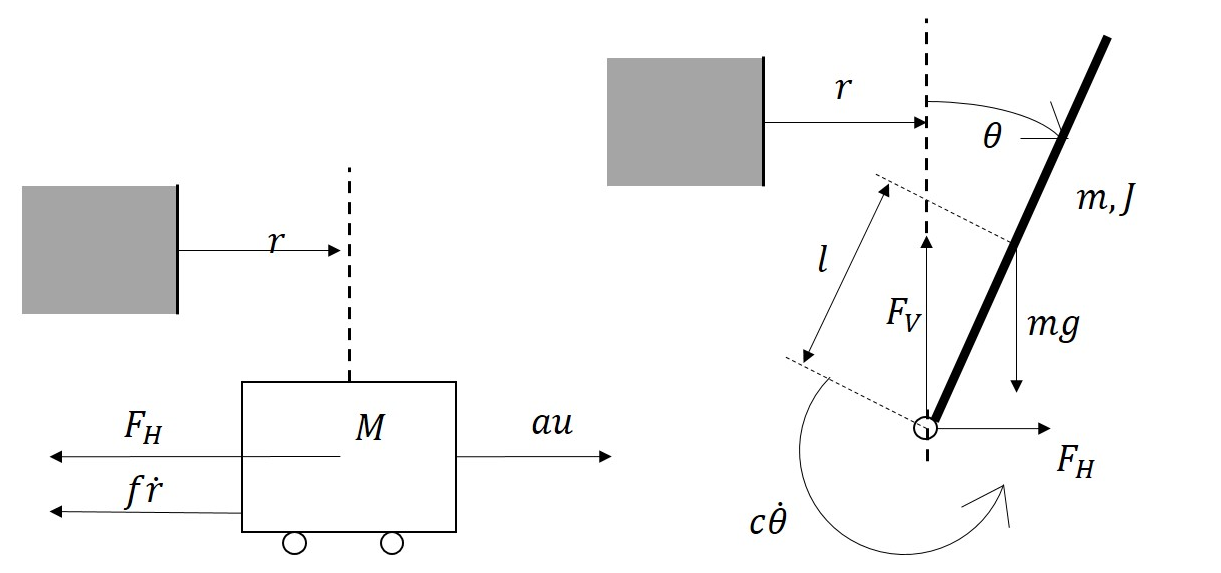
\includegraphics[width=0.6\linewidth]{modeling.eps}
        \caption{図\ref{modeling}: モデリングのための力の分解}
        \label{modeling}
    \end{center}
\end{figure}

図\ref{modeling}から導出した倒立振子系の運動方程式を
式(\ref{modeling:cart1})から式(\ref{modeling:pend2})に示す.

\begin{equation}
    M \ddot{r} = au - F_{H} - f \dot{r}
    \label{modeling:cart1}
\end{equation}
\begin{equation}
    J \ddot{\theta} = lF_{V}\sin{\theta} - lF_{H}\cos{\theta} - c \dot{\theta}
    \label{modeling:pend1}
\end{equation}
\begin{equation}
    m\frac{d^2}{dt^2}(r + l\sin{\theta}) = F_{H}
    \label{modeling:cart2}
\end{equation}
\begin{equation}
    m\frac{d^2}{dt^2}(l\cos{\theta}) = F_{V} - mg
    \label{modeling:pend2}
\end{equation}

ただし,$M$,$f$は台車の質量と摩擦係数,$m$,$l$,$c$,$J$は振子の質量,振子の重心から回転軸までの距離,
回転軸摩擦係数,重心周りに働く慣性モーメントである.また,$F_{H}$,$F_{V}$は振子が台車から受ける
水平効力と垂直抗力である.$F$はモータによる台車への駆動力であり,定数$a$,駆動アンプへの入力電圧$u$を用いて
式(\ref{F})で表される.

\begin{equation}
    F = au
    \label{F}
\end{equation}

ここで,系の状態$x$を4つの状態変数からなる縦ベクトルとする.すなわち,
$$
    x = \left[
    \begin{array}{c}
        r \\
        \theta \\
        \dot{r} \\
        \dot{\theta}
    \end{array}
    \right]
$$
と定義する.
次に,式(\ref{modeling:cart1})から式(\ref{modeling:pend2})から倒立振子系の非線形方程式を求める.
式(\ref{modeling:cart1}),式(\ref{modeling:pend1})から$F_{H}$を消去すると,式(\ref{del_Fh})が得られる.

\begin{equation}
    (M + m) \ddot{r} + (ml\cos{\theta}) \ddot{\theta} = au + (ml\sin{\theta}) \dot{\theta}^2 - f \dot{r}
    \label{del_Fh}
\end{equation}

また,式(\ref{modeling:pend1}),式(\ref{modeling:cart2}),式(\ref{modeling:pend2})から
$F_{H}$,$F_{V}$を消去すると,

$$
    J \ddot \theta = l\left(
        m\frac{d^2}{dt^2}\left(
            l\cos{\theta} + mg
            \right)
        \right)\sin{\theta}
        -
        l\left(
            m\frac{d^2}{dt^2}\left(
                r + l\sin{\theta}
            \right)
        \right)\cos{\theta}
$$

となり,式(\ref{del_Fh_Fv})が得られる.

\begin{equation}
    ml\cos{\theta} \ddot{r} + (J + ml^2) \ddot{\theta} = mgl\sin{\theta} -c \dot{\theta}
    \label{del_Fh_Fv}
\end{equation}

式(\ref{del_Fh}),式(\ref{del_Fh_Fv})を行列表現すると,

$$
    % --- left side --- %
    % --- Matrix first --- %
    \left[
    \begin{array}{cc}
        M + m          &  ml\cos{\theta} \\
        ml\cos{\theta}  &  J + ml^2
    \end{array}
    \right]
    % --- Matrix second --- %
    \left[
    \begin{array}{c}
        \ddot{r} \\
        \ddot{\theta}
    \end{array}    
    \right]
    =
    % --- right side --- %
    \left[
        \begin{array}{c}
            -f \dot{r} + ml(\sin{\theta)} \dot{\theta}^2 + au \\
            mgl\sin{\theta} - c \dot{\theta}
        \end{array}
    \right]
$$

$$
    % --- left side --- %
    \left[
    \begin{array}{c}
        \ddot{r} \\
        \ddot{\theta}
    \end{array}    
    \right]
    =
    % --- right side --- %
    % --- Matrix first --- %
    \left[
    \begin{array}{cc}
        M + m           &  ml\cos{\theta} \\
        ml\cos{\theta}  &  J + ml^2
    \end{array}
    \right]^{-1}
    % --- Matrix second --- %
    \left[
        \begin{array}{c}
            -f \dot{r} + ml(\sin{\theta)} \dot{\theta}^2 + au \\
            mgl\sin{\theta} - c \dot{\theta}
        \end{array}
    \right]
$$

となる.よって,

\begin{equation}
    \dot x = f(x, u) = 
    \left[
        \begin{array}{c}
            \dot{r} \\
            \dot{\theta} \\
            K^{-1}
            \left[
                \begin{array}{c}
                    -f \dot{r} + ml(\sin{\theta}) \dot{\theta}^2 + au \\
                    mgl\sin{\theta} - c \dot{\theta}
                \end{array}
            \right]
        \end{array}    
    \right],\
    K = 
    \left[
        \begin{array}{cc}
            M + m           &  ml\cos{\theta} \\
            ml\cos{\theta}  &  J + ml^2
        \end{array}
    \right]
    \label{nonlinear}
\end{equation}

が得られる.本実験では,不安定平衡点$x=0$近傍で線形化したモデルを採用できる.
$\theta$に関して式(\ref{nonlinear})を一次近似すると,
$\sin{\theta} \approx \theta,\ \cos{\theta} \approx 1,\ \theta^2 \approx 0$と近似できることから,

\begin{equation}
% --- Matrix x_dot --- %
    \dot x = 
    \left[
        \begin{array}{c}
            \dot{r} \\
            \dot{\theta} \\
            K^{-1}
            \left[
                \begin{array}{c}
                    -f \dot{r} + au \\
                    mgl \theta - c \dot{\theta}
                \end{array}
            \right]
        \end{array}    
    \right],\
    %--- Matrix K ---%
    K = 
    \left[
        \begin{array}{cc}
            M + m  &  ml \\
            ml     &  J + ml^2
        \end{array}
    \right]
    \label{linear_k}
\end{equation}

を得る.線形化された倒立振子系の状態方程式は,式(\ref{linear_general})のように表現される.

\begin{equation}
    \dot x = Ax + Bu
    \label{linear_general}
\end{equation}

ここで,

$$
    % --- Matrix A --- %
    A = 
    \left[
        \begin{array}{cc}
            O_{2 \times 2}  &  I_{2} \\
            A_{21}          &  A_{22}
        \end{array}
    \right],\
    % --- Matrix B --- %
    B = 
     \left[
        \begin{array}{c}
            O_{2 \times 1} \\
            B_{2}
        \end{array}
    \right]
$$

である.ただし,

$$
    A_{21} = K^{-1}
    \left[
        \begin{array}{cc}
            0  &  0 \\
            0  &  mgl
        \end{array}    
    \right],\
    A_{22} = K^{-1}
    \left[
        \begin{array}{cc}
            -f  &  0 \\
            0   &  -c
        \end{array}    
    \right],\
    B_{2} = K^{-1}
    \left[
        \begin{array}{c}
            a \\
            0
        \end{array}    
    \right]
$$

である.

\subsection{観測方程式}
2つの観測出力は,

$$
    y_{1} = c_{1} r
$$

$$
    y_{2} = c_{2} \theta
$$

のように表される.ここで,$c_{1}$は変位・電圧変換係数, $c_{2}$は角度・電圧変換係数である.
これらからなる縦ベクトル,すなわち出力$y$を,

$$
    y = 
    \left[
        \begin{array}{c}
            y_{1} \\
            y_{2}
        \end{array}    
    \right]
$$

と定義すると,倒立振子系に対する観測方程式を,

\begin{equation}
    y = Cx
\end{equation}

と表せる.ただし,

$$
    % --- Matrix N --- %
    N = 
    \left[
        \begin{array}{cc}
            c_{1}  &  0 \\
            0      &  c_{2}
        \end{array}
    \right],\
    % --- Matrix C --- %
    C = 
    \left[
        \begin{array}{cc}
            N  &  O_{2 \times 2}
        \end{array}
    \right]
    =
    \left[
        \begin{array}{cccc}
            c_{1}  &    0    &    0    &    0 \\
            0      &  c_{2}  &    0    &    0
        \end{array}
    \right]
$$

である.

\section{パラメータの同定}
パラメータの同定のため,以下の手順で測定を行う.

\begin{enumerate}
    \item 実測できるパラメータ$m$(振子の質量[kg]),$l$(振子の重心から回転軸までの長さ[m])の測定を行う.
    \item 駆動アンプへの入力電圧とモータ駆動力の変換係数$a$を求める.
    \begin{enumerate}
        \item 振子を台車から取り外す.
        \item モータに一定電圧$u$を加え,ばねばかりで引き,台車が正の方向に動き始めるときの力($au+$摩擦力)
        を$f_{max}$,負の方向に動き始めるときの力($au-$摩擦力)を$f_{min}$とする.測定は
        $10$[V], $11$[V], ..., $15$[V]の各電圧に対して行う.
        \item $f_{max}$, $f_{min}$それぞれの回帰直線の傾きを平均し,その値を$a$[N/V],
        すなわち入力電圧$u$[V]とモータ駆動力$f$[N]の変換係数とする.
        \begin{figure}[htbp]
            \begin{center}
                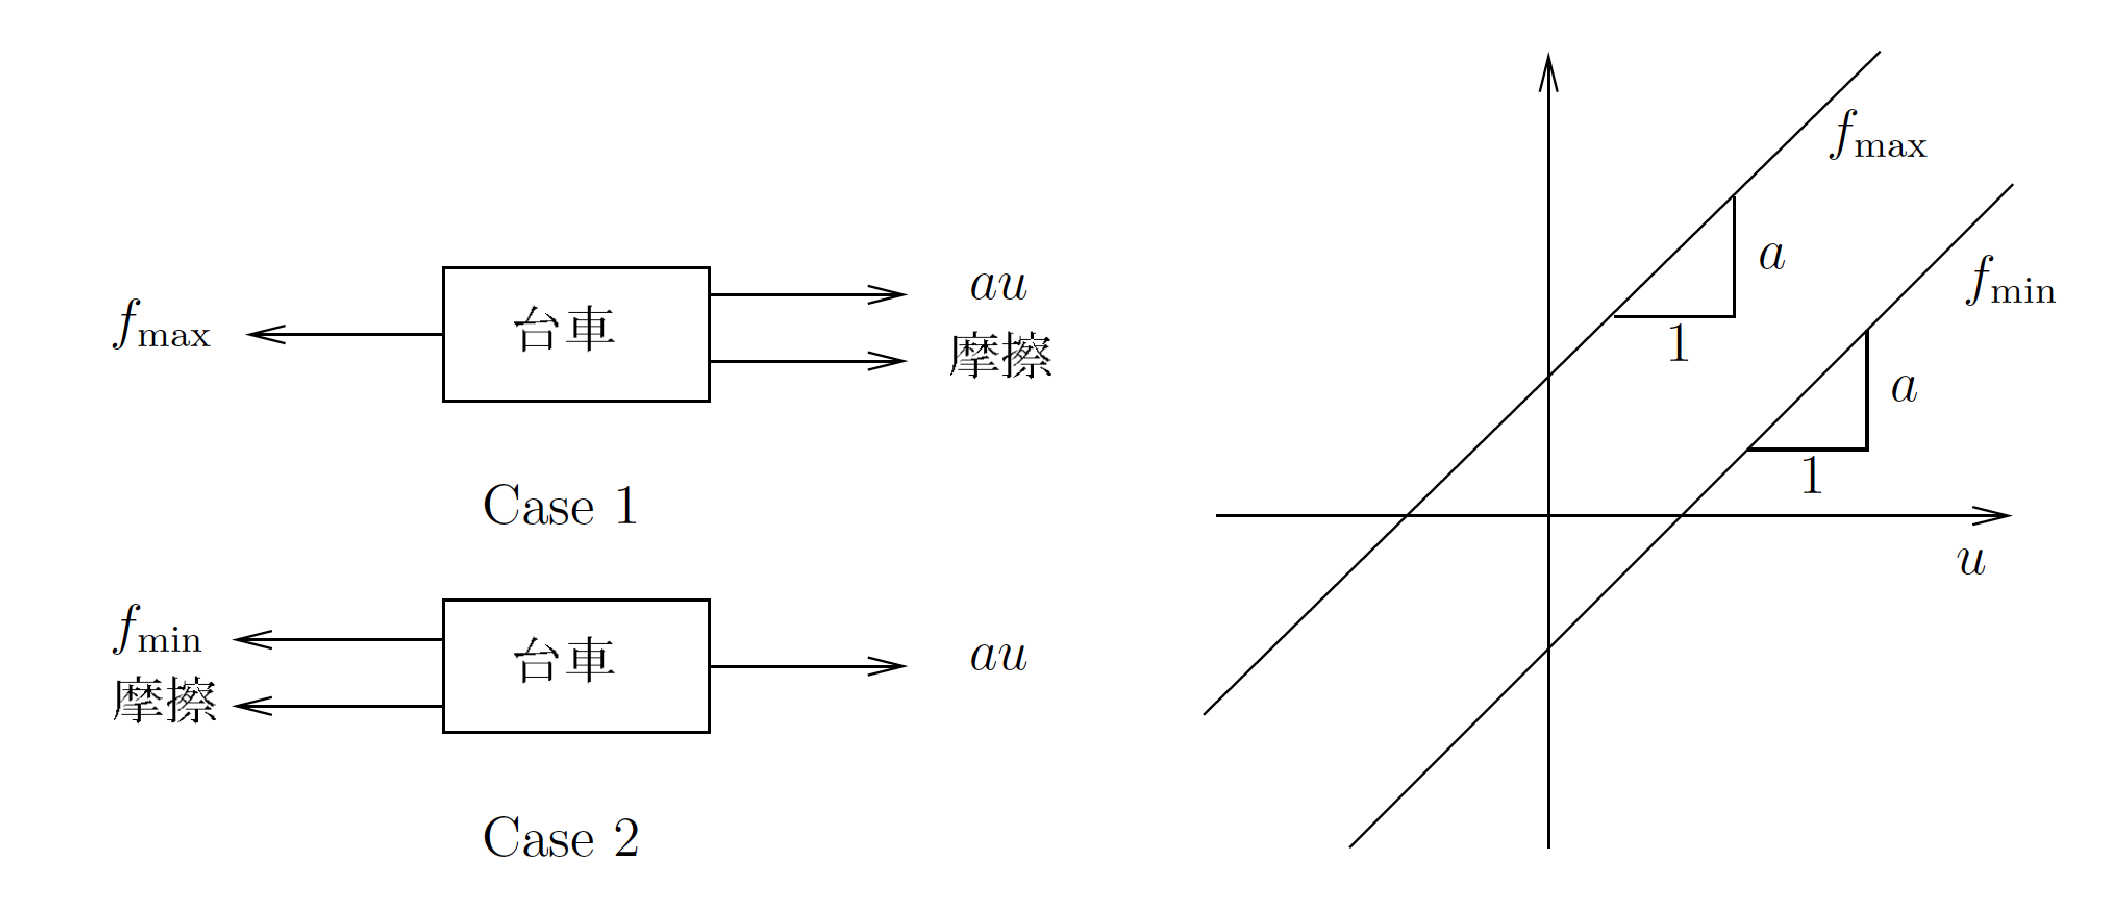
\includegraphics[width=0.6\linewidth]{definition_a.eps}
                \caption{図\ref{definition_a}: パラメータ$a$の決定}
                \label{definition_a}
            \end{center}
        \end{figure}
    \end{enumerate}

    \item 台車の変位$r$と$y_{1}$の変換係数を$c_{1} = 1.0$ [V/m], 
    振子の角度$\theta$と$y_{2}$の変換係数を$c_{2} = 1.0$ [V/rad]とする.

    \item 以下の2通りの方法で台車系の質量$M$[kg]と摩擦係数$f$[kg/s]を求める.
    \begin{itemize}
        % --- step response --- %
        \item ステップ応答による方法 \\
        \quad 振子を台車から取り外したまま,台車のステップ応答を測定する.そのとき,台車の運動方程式は,

        \begin{equation}
            M \ddot r = au - fr
            \label{eq_model}
        \end{equation}

        であり,入力$u$から目標値$r$までの伝達関数$G$は,

        \begin{equation}
            G(s) = \frac{K}{s(Ts + 1)}
        \end{equation}

        となる.ただし,

        \begin{equation}
            K = \frac{a}{f},\ T = \frac{M}{f}
        \end{equation}

        である.初期状態を零ベクトルとすれば,台車のステップ応答は,

        \begin{equation}
            r(t) = KU_{0}
            \left(
                T\exp \left(\frac{-t}{T} \right) + t - T
            \right)
            \label{step_response}
        \end{equation}

        である.(図\ref{cart_step}参照)ただし,$U_{0}$はステップ入力の$t > 0$での値である.式(\ref{step_response})
        において,$t \to \infty$の極限をとると,

        \begin{equation}
            \lim_{t \to \infty} r(t) = KU_{0}(t - T)
            \label{lim_step_response}
        \end{equation}

        となる.図\ref{cart_step}を参考に,式(\ref{lim_step_response})から$T$, $K$を求め,

        \begin{figure}[htbp]
            \begin{center}
                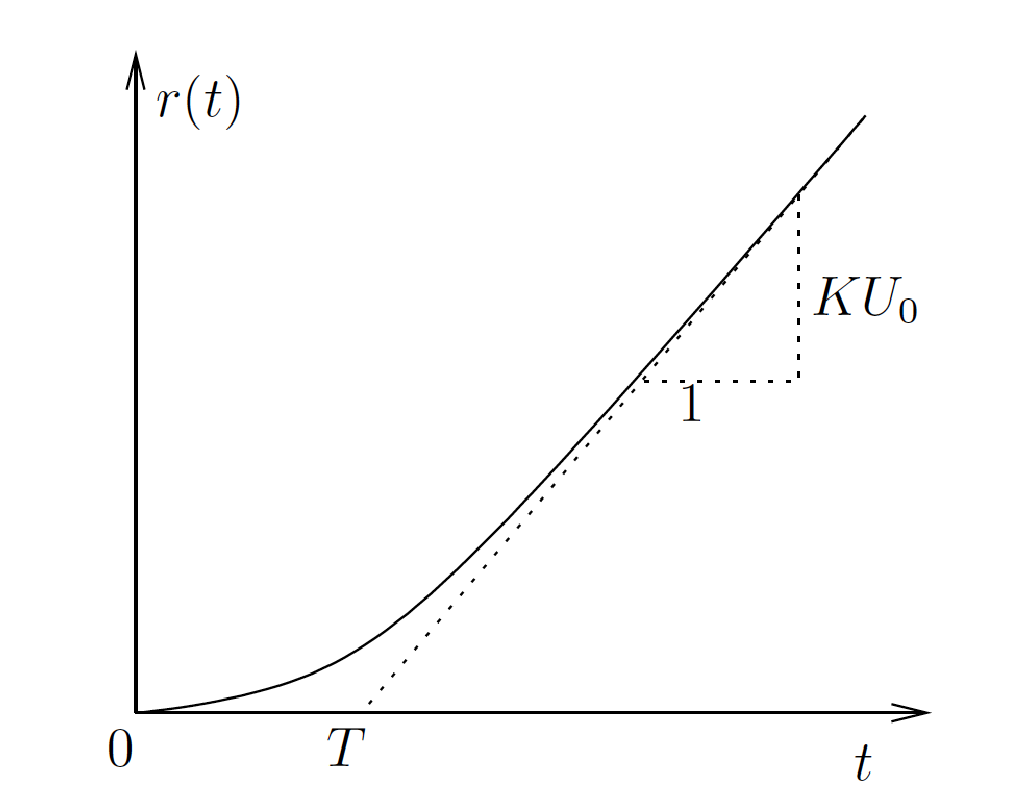
\includegraphics[width=0.6\linewidth]{cart_step.eps}
                \caption{図\ref{cart_step}: 台車のステップ応答}
                \label{cart_step}
            \end{center}
        \end{figure}

        $10$[V], $11$[V], ..., $15$[V]の各電圧をステップ入力として与え,それぞれのステップ応答
        から求めたパラメータ$T$, $K$を平均し,$M$, $f$を決定する.

        % --- feedback --- %
        \newpage
        \item フィードバックによる方法 \\
        \quad 台車の数式モデルである式(\ref{eq_model}),出力$y_{1} = c_{1}r$について,フィードバックにより
        入力を制御する.すなわち,

        \begin{equation}
            u = k(y_{c} - y_{1})
        \end{equation}

        とする($y_{c} =$ const, $k > 0$).このとき,閉ループシステムの応答は,

        \begin{equation}
            M \ddot{y_{1}} + f \dot{y_{1}} + c_{1}aky_{1} = c_{1}aky_{c}
        \end{equation}

        となる(図\ref{feedback}参照).一方,偏差$z$を加え,ばねばかりで引き,台車が正の方向に動き始めるときの力

        \begin{equation}
            z = y_{1} - y_{c}
        \end{equation}

        により定義すると,$z$は以下の式(\ref{secondary_system})に従う.

        \begin{equation}
            \ddot{z} + 2\zeta \omega_{n} \dot{z} + \omega_{n}^2 z = 0
            \label{secondary_system}
        \end{equation}

        ただし,

        \begin{equation}
            \zeta = \frac{f}{2\sqrt{c_{1}akM}},\ \omega_{n} = \sqrt{\frac{c_{1}ak}{M}}
            \label{zeta}
        \end{equation}

        である.式(\ref{secondary_system})の解は,

        $$
            0 < \zeta < 1
        $$

        のとき減衰振動となり,そのときの解は,

        $$
            z(t) = \frac{z_{0}}{\sqrt{1 - \zeta^2}} \exp(-\omega_{n} \zeta t)
            \sin{\left( \omega_{n} \sqrt{1 - \zeta^2}t + \phi \right)}
        $$

        ただし,
        
        $$
            \phi = \tan^{-1}{\frac{\sqrt{1 - \zeta^2}}{\zeta}}
        $$

        で与えられる.ここで,$z_{0} = z(0) = -y_{c}$である.いま,$T$とし,時刻$t_{1}$と$t_{2} = t_{1} + T$
        において波形$z$の山が隣り合うものとする.このとき.振幅の減衰比は,

        \begin{equation}
            \frac{|z_{2}(t_{2})|}{z_{2}(t_{1})} = \exp(-\lambda)
        \end{equation}

        となる.$\lambda$は対数減衰比であり,次が成り立つ.

        \begin{equation}
            \lambda = \frac{2\pi \zeta}{\sqrt{1 - \zeta^2}},\
            T = \frac{2\pi}{\omega_{n} \sqrt{1 - \zeta^2}}
            \label{lambda}
        \end{equation}

        従って,式(\ref{zeta}), 式(\ref{lambda})から,パラメータ$M$, $f$は,

        \begin{equation}
            M = \frac{c_{1}akT^2}{4\pi^2 + \lambda^2},\
            f = \frac{2\lambda M}{T}
        \end{equation}

        のようにして求まる.

        \begin{figure}[htbp]
            \begin{center}
                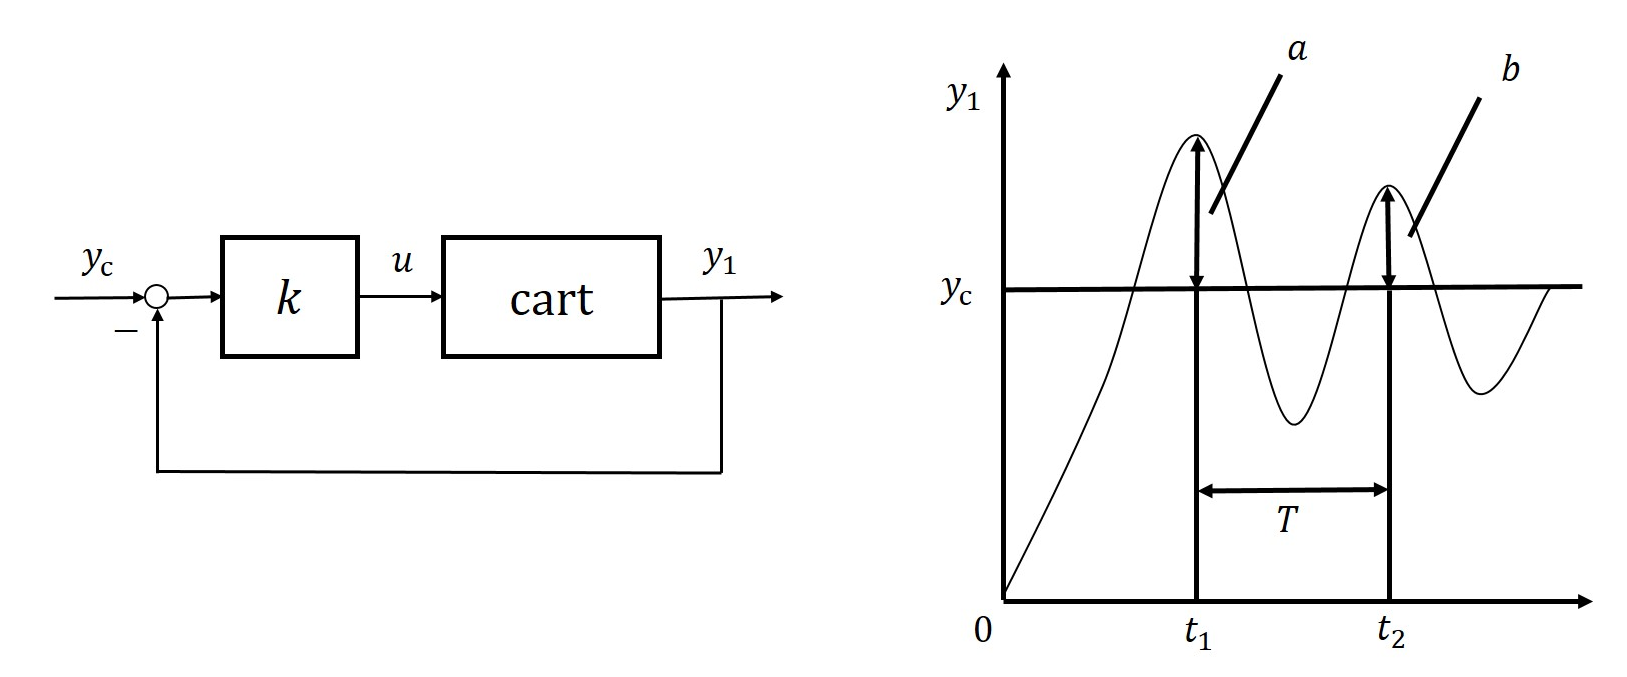
\includegraphics[width=0.6\linewidth]{feedback.eps}
                \caption{図\ref{feedback}: 台車のステップ応答}
                \label{feedback}
            \end{center}
        \end{figure}

    \end{itemize}

    \item パラメータ$J$と$c$の決定 \\
    \quad 振子を台車に取り付け,台車を固定したまま振子を自由振動させることにより,パラメータ$J$, $c$を測定する.
    このとき,振子の運動方程式は,

    \begin{equation}
        (J + ml^2) \ddot{\theta} = -mgl\sin{\theta} - c \dot{\theta}
        \label{pend_eq1}
    \end{equation}

    \begin{equation}
        y_{2} = c_{2} \theta
        \label{pend_eq2}
    \end{equation}

    で与えられる.$\theta$を微小区間で考えると,式(\ref{pend_eq1}), 式(\ref{pend_eq2})は次のように書ける.

    \begin{equation}
        \ddot{y_2} + 2\zeta \omega_{n} \dot{y_{2}} + \omega_{n}^2y_{2} = 0
        \label{pend_eq3}
    \end{equation}

    \begin{equation}
        \zeta = \frac{c}{2\sqrt{mgl(J + ml^2)}},\
        \omega_{n} = \sqrt{\frac{mgl}{J + ml^2}}
    \end{equation}

    式(\ref{pend_eq3})の解で表される減衰振動の対数減衰率を$\lambda$, 周期を$T$とすると,式(\ref{lambda})
    が成り立つことから$J$と$c$は,

    \begin{equation}
        J = \frac{mglT^2}{4\pi^2 + \lambda^2} - ml^2,\
        c = \frac{2\lambda (J + ml^2)}{T}
    \end{equation}

    のように与えられる.

\end{enumerate}


\subsection{パラメータの検証}
測定した物理パラメータを表\ref{pend_params}に示す。

\begin{table}[htbp]
    \begin{center}
        \caption{表\ref{pend_params}: 測定した物理パラメータ}
        \begin{tabular}{|l|r|} \hline
            $m$ $[\mathrm{kg}]$ & 0.038 \\ \hline
            $l$ $[\mathrm{m}]$ & 0.12 \\ \hline
            $M(\rm{Step})$ $[\mathrm{kg}]$ & 1.00 \\ \hline
            $f(\rm{Step})$ $[\mathrm{kg/s}]$ & 9.67 \\ \hline
            $M(\rm{Feedback})$ $[\mathrm{kg}]$ & 1.51 \\ \hline
            $f(\rm{Feedback})$ $[\mathrm{kg/s}]$ & 16.5 \\ \hline
            $J$ $[\mathrm{kg \cdot m^2}]$ & 3.90E-4 \\ \hline
            $c$ $[\mathrm{kg \cdot m^2/s}]$ & 9.82E-5 \\ \hline
            $a$ $[\mathrm{N/V}]$ & 0.49 \\ \hline
            $c_1$ $[\mathrm{V/m}]$ & 1.0 \\ \hline
            $c_2$ $[\mathrm{V/rad}]$ & 1.0 \\ \hline
            $g$ $[\mathrm{m/s^2}]$ & 9.8 \\ \hline
        \end{tabular}
        \label{pend_params}
    \end{center}
\end{table}

次に、表\ref{pend_params}に示すパラメータの検証を行う。

\subsection{$M$と$f$の検証}
図\ref{step13_correct}に、入力電圧$13.0$[V]のときの台車系のステップ応答とそのシミュレーションを示す。
また、図\ref{feedback_correct}に台車系のフィードバック応答とそのシミュレーションを示す。

\begin{figure}[htbp]
    \begin{center}
        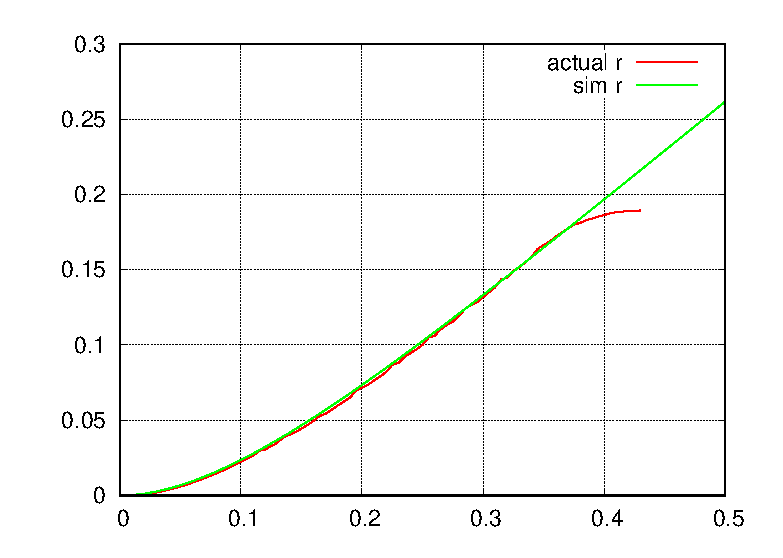
\includegraphics[width=0.6\linewidth]{step13_correct.eps}
        \caption{図\ref{step13_correct}: ステップ応答による$M$と$f$の検証}
        \label{step13_correct}
    \end{center}
\end{figure}

\begin{figure}[htbp]
    \begin{center}
        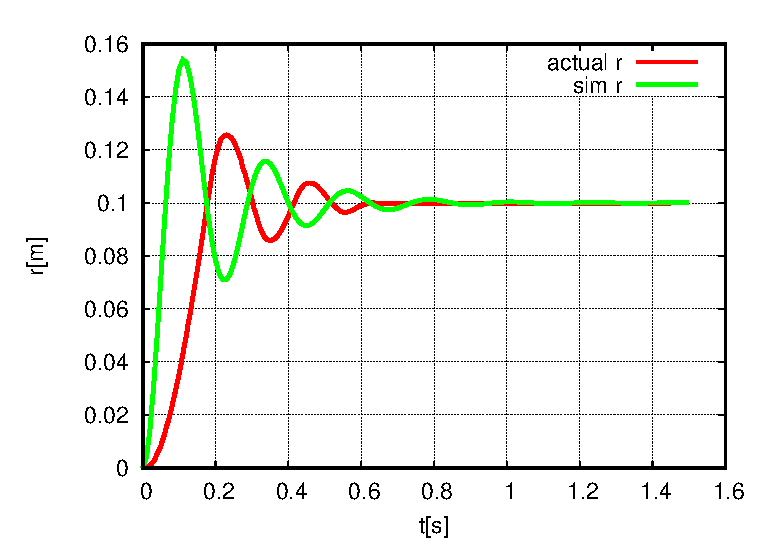
\includegraphics[width=0.6\linewidth]{feedback_correct.eps}
        \caption{図\ref{feedback_correct}: ステップ応答による$M$と$f$の検証}
        \label{feedback_correct}
    \end{center}
\end{figure}

図\ref{feedback_correct}では、シミュレーション結果と実験結果が不一致なため、不適切んばパラメータ
である。一方、図\ref{step13_correct}では、直線近似を行うために十分な一致が見られるため、
ステップ応答により測定した$M = 1.00$と$f = 9.67$を用いて実験を行う。

\subsection{$J$と$c$の検証}
図\ref{jc_correct}に振子の自由振動の応答とそのシミュレーションを示す。
実験とシミュレーションの波形を比較すると、初期位相が異なっているが、振幅と周期が近しい値をとっているので
測定した$J$ = 3.90E-4と$c$ = 9.82E-5を実験に用いる。

\begin{figure}[htbp]
    \begin{center}
        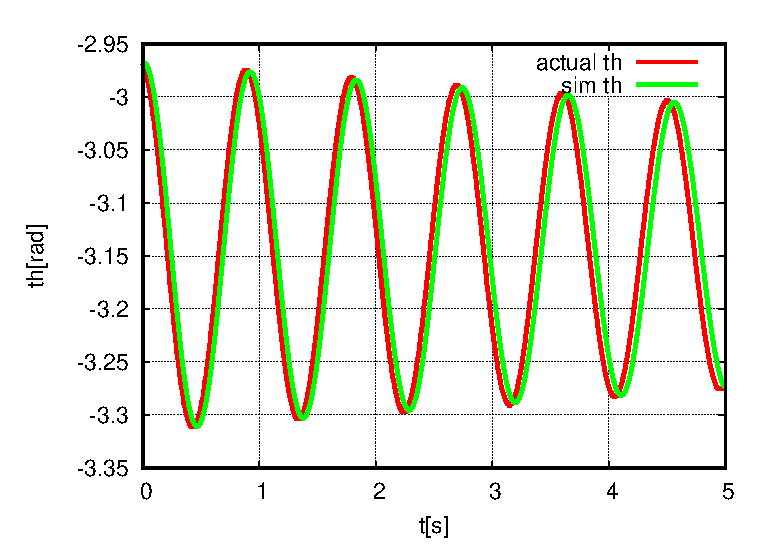
\includegraphics[width=0.6\linewidth]{jc_correct.eps}
        \caption{図\ref{jc_correct}: 自由振動による$J$と$c$の検証}
        \label{jc_correct}
    \end{center}
\end{figure}



% =============================== chapter 2 END =============================== %
% --- Chapter 2 END --- %

% ----- chapter 3 ----- %
% ================================= chapter 3 ================================= %
\chapter{制御系設計}
\subsection{特性解析}
第\ref{chapter_modeling}章で物理パラメータの決定と数式モデルの導出を行った.
ここでは,決定したパラメータから,式(\ref{linear_k}),式(\ref{linear_general})の特性解析を行う.
倒立振子の線形モデルの状態空間表現は以下のようになる.

\begin{equation}
    A,\ B,\ Cの値
    \label{ABC}
\end{equation}

まず,行列$A$の安定判別を行う.$A$のすべての固有値に関して,実部が負であれば$A$は安定性行列である.
すなわち,$A$の固有値$\lambda_{1}$, $\lambda_{2}$, $...$に対し,

$$
    \mbox{Re}[\lambda_{i}] < 0
$$

が成立すればよい.\MaTX{}で$A$の固有値を算出した結果を表\ref{eigen_A}に示す.

\begin{table}[htbp]
    \begin{center}
        \caption{表\ref{eigen_A}: $A$の固有値}
        \begin{tabular}{|c|c|} \hline
            固有値 & Re[$\lambda_{i}$] \\ \hline \hline
            0 & 0 \\ \hline
            0 & 0 \\ \hline
            0 & 0 \\ \hline
            0 & 0 \\ \hline
        \end{tabular}
        \label{eigen_A}
    \end{center}
\end{table}

表\ref{eigen_A}から,倒立振子系のシステムは不安定である.次に,システムの可制御性,可観測性を判別する.
可制御性は,$n$をシステムの次数(倒立振子系のシステムの次数は$n = 4$)に対し,可制御性行列,

$$
    U_{C} =
    \left[
        \begin{array}{ccccc}
            B  &  AB  &  A^2B  &  \dots  &  A^{n-1}B
        \end{array}
    \right]
$$

のランクがシステムの次数と等しければ満たされる.また,可観測性行列は,

$$
    U_{o} = 
    \left[
        \begin{array}{c}
            C \\
            CA \\
            CA^2 \\
            \vdots \\
            CA^{n-1}
        \end{array}
    \right]
$$

であり,$U_{o}$のランクがシステムの次数と等しければ可観測となる.
式(\ref{ABC})において,\MaTX{}を用いて$U_{c}$, $U_{o}$のランクを計算した結果,以下のようになった.

$$
    Uc, Uoのランク
$$

以上から,倒立振子系のシステムは不安定であり,可制御,可観測である.

\subsection{制御システムの構成}
図\ref{controller_system}に,倒立振子系に対する制御システムの構成を示す.

\begin{figure}[htbp]
    \begin{center}
        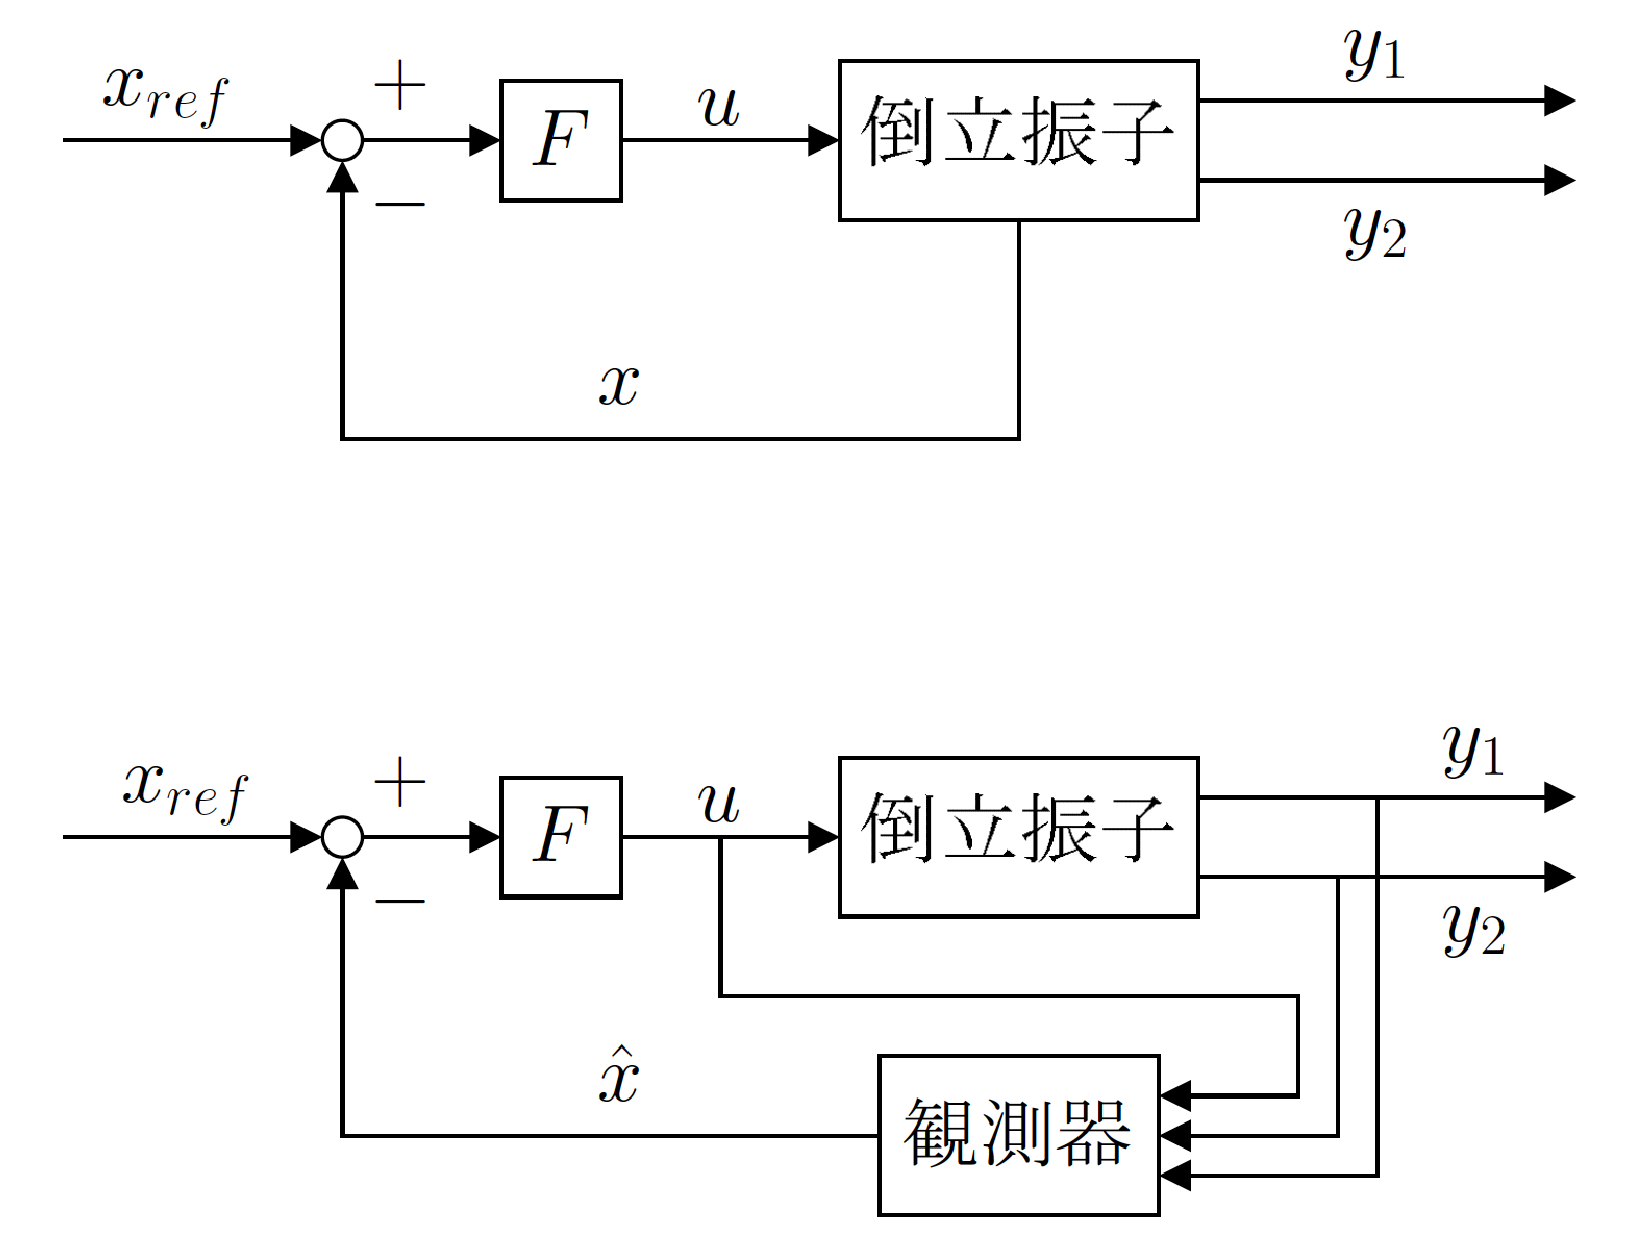
\includegraphics[width=0.6\linewidth]{controller_system.eps}
        \caption{図\ref{controller_system}: 制御システムの構成}
        \label{controller_system}
    \end{center}
\end{figure}

制御系のフィードバックによる入力は,

$$
    u = -F \left( x - x_{ref} \right)
$$

ただし,

$$
    x_{ref} =
    \left[
        \begin{array}{c}
            y_{c} \\
            0 \\
            0 \\
            0
        \end{array}
    \right]
$$

であり,$y_{C}$は指定された台車位置を表す.本実験では,$\dot{r}$, $\dot{\theta}$の検出器は
用いず,状態$x$は推定値$\hat{x}$において,

\begin{equation}
    x = \lim_{t \to \infty} \hat{x}
    \label{definition_x}
\end{equation}

とする.また,式(\ref{definition_x})を満足する最小次元オブザーバ,

\begin{equation}
    \hat{z} = \hat{A}z + \hat{B}y + \hat{J}u
    \label{z_hat}
\end{equation}

\begin{equation}
    \hat{x} = \hat{C}z + \hat{D}y
    \label{x_hat}
\end{equation}

を用いる.ここで,オブザーバの次数は$2$であり,設計すべき制御システムは以下のようになる.

\begin{itemize}
    \item $F(1 \times 4)$
    \item $\hat{A}(2 \times 2)$, $\hat{B}(2 \times 2)$, 
    $\hat{J}(2 \times 1)$, $\hat{C}(4 \times 2)$, $\hat{D}(4 \times 2)$
\end{itemize}


\subsection{状態フィードバック$F$の設計}
$F$は,システムを安定化する状態フィードバック,

\begin{equation}
    u = -Fx
    \label{feedback_u}
\end{equation}

を満たすように求める.式(\ref{feedback_u})をLQ問題として解くため,$2$次形式評価関数,

\begin{equation}
    J = \int_{0}^{\infty}
    \left(
        x^{T}Qx + Ru^2
    \right)
    dt
    \label{eval2_J}
\end{equation}

\begin{equation}
    Q = \mbox{diag}(q_{1}^2, q_{2}^2, q_{3}^2, q_{4}^2), R = 1
    \label{eval2_Q}
\end{equation}

を考える.ここで,$\mbox{diag}(\dots)$は,各引数を固有値にもつ対角行列を表す.これは,

\begin{equation}
    J = \int_{0}^{\infty}
    \left(
        q_{1}^2 r^2 + q_{2}^2 \theta^2 + q_{3}^2 \dot{r}^2 + q_{4}^2 \dot{\theta}^2 + u^2
    \right)
    dt
\end{equation}

と表せるから,$q_{1}$, $q_{2}$, $q_{3}$, $q_{4}$はそれぞれ,台車位置$r$, 振子角度$\theta$,
台車速度$\dot{r}$, 振子角速度$\dot{\theta}$に対する重み係数である.
式(\ref{eval2_J}), 式(\ref{eval2_Q})を最小にする$F$は,リッカチ方程式,

$$
    A^{T}P + PA - PBR^{-1}B^{T}P + Q = 0
$$

の解$(P > 0)$に対し,

$$
    F = R^{-1}B^{T}P
$$

で与えられる.

\subsection{$\hat{A}$, $\hat{B}$, $\hat{C}$, $\hat{D}$, $\hat{J}$の設計}
式(\ref{z_hat}), 式(\ref{x_hat})が式(\ref{definition_x})を満足するための十分条件は,
ある行列$U(1 \times 4)$が存在して,

$$
    \begin{array}{c}
        UA = \hat{A}U + \hat{B}C \\
        UB = \hat{J} \\
        I = \hat{C}U + \hat{D}C
    \end{array}
$$

であり,かつ$\hat{A}$が安定性行列であることである.これらの条件を満足するオブザーバを設計するため,
Gopinathの方法を用いる.

\subsection{制御システムの離散化}
式(\ref{feedback_u}), 式(\ref{z_hat}), 式(\ref{x_hat})で示した$u,\ \hat{z},\ \hat{x}$は,
連続時間上で設計される制御器である.そこで,計算機で制御器を表現するためこれらの離散時間化を行う.
各サンプリングの間隔を$\Delta$とすると,

$$
    \begin{array}{c}
        u[k] = -F \hat{x}[k] \\
        z[k + 1] = \hat{A}_{d}z[k] + \hat{B}_{d}y[k] + \hat{J}_{d}u[k] \\
        \hat{x}[k] = \hat{C}_{d}z[k] + \hat{D}_{d}y[k]
    \end{array}
$$

と表せる.ただし,$k = 0, 1, \dots$において,

$$
    x_{ref} = 
    \left[
        \begin{array}{cc}
            \hat{A}_{d}  &  \left[
                                \begin{array}{cc}
                                    \hat{B}_{d}  &  \hat{J}_{d}
                                \end{array}
                            \right] \\
            0            &  I_{3}
        \end{array}
    \right]
    =
    \exp \Delta
    \left[
        \begin{array}{cc}
            \hat{A}  &  \left[
                            \begin{array}{cc}
                                \hat{B}  &  \hat{J}
                            \end{array}
                        \right] \\
            0        &  I_{3}
        \end{array}
    \right]
$$

である.

\subsection{振り上げ制御と安定化}
台車と振子の運動方程式は,式(\ref{del_Fh}), 式(\ref{del_Fh_Fv})から,

$$
    \begin{array}{c}
        (M + m) \ddot{r} + (ml\cos{\theta}) \ddot{\theta} 
            = au + (ml\sin{\theta}) \dot{\theta}^2 - f \dot{r} \\
        ml\cos{\theta} \ddot{r} + (J + ml^2) \ddot{\theta} 
            = mgl\sin{\theta} -c \dot{\theta}
    \end{array}
$$

で与えられる.振子が鉛直上向きのときを基準とする振子の力学的エネルギーは,

\begin{equation}
    E = \frac{1}{2} \left( J + ml^2 \right) \ddot{\theta}
        + mgl \left( \cos{\theta} - 1 \right)
\end{equation}

であり,力学的エネルギーの時間微分は,

\begin{equation}
    \frac{dE}{dt} = (J + ml) \theta \ddot{\theta}
                    - mgl \dot{\theta} \sin{\theta}
    \label{dEdt}
\end{equation}

となる.振り上げ処理を行うため,入力$u$を次のように計算する.

\begin{equation}
    u = \frac{1}{a}
        \left(
            f \dot{r} - ml \sin{\theta} \dot{\theta}^2 + ml \cos{\theta} \ddot{\theta}
            + (M + m)v
        \right)
    \label{swing_u}
\end{equation}

\begin{equation}
    v = - \frac{c \dot{\theta}}{ml\cos{\theta}} 
        + k(E - E_{0}) \mbox{sign}(\dot{\theta}\cos{\theta})
    \label{swing_v}
\end{equation}

$\mbox{sign}$は符号関数であり,引数が$0$のとき$0$を,正のとき$1$を,負のとき$-1$を返す.
式(\ref{del_Fh})に式(\ref{swing_u})を代入すると,

\begin{equation}
    \ddot{r} = v
    \label{ddot_r}
\end{equation}

を得る.式(\ref{ddot_r}), 式(\ref{swing_v})を式(\ref{del_Fh_Fv})に代入すると,

\begin{equation}
    (J + ml^2) \ddot{\theta} = mgl \sin{\theta}
                - ml \cos{\theta} (k(E - E_{0}) \mbox{sign} (\dot{\theta} \cos{\theta}))    
\end{equation}

を得る.さらに,これを式(\ref{dEdt})に代入すると,

\begin{equation*}
    \begin{split}
        \frac{dE}{dt} &= -ml \dot{\theta} \cos{\theta} (k(E - E_{0}) 
                            \mbox{sign} (\dot{\theta} \cos{\theta})) \\
                      &= -mlk(E - E_{0}) \mbox{sign} (\dot{\theta} \cos{\theta}) \dot{\theta} (\cos{\theta})
    \end{split}
\end{equation*}

となる.リアプノフ関数として,

\begin{equation}
    V = \frac{(E - E_{0})^2}{2}
\end{equation}

を考えると,$V$の時間微分,

\begin{equation}
    \begin{split}
        \frac{dV}{dt} &= (E - E_{0}) \frac{dE}{dt} \\
                      &= -mlk(E - E_{0})^2 \mbox{sign} (\dot{\theta} \cos{\theta}) \dot{\theta} (\cos{\theta}) \leq 0
    \end{split}
\end{equation}

これより,$\dot{\theta} \cos{\theta} \neq 0$のとき,$V$は減少して$0$に収束し,$E$は$E_{0}$に収束する.
実際の制御では,台車の加速度目標$v$を制限し,

$$
    u = \frac{1}{a}
        \left(
            f \dot{r} - ml \sin{\theta} \dot{\theta}^2 + ml \cos{\theta} \ddot{\theta}
            + (M + m)v
        \right)
$$

$$
    v = - \frac{c \dot{\theta}}{ml\cos{\theta}} 
        + \mbox{sat}_{ng} (k(E - E_{0}) \mbox{sign}(\dot{\theta}\cos{\theta}))
$$

とする.ただし,$\mbox{sat}_{ng}$は最小値$-ng$, 最大値$ng$の飽和関数である.また,$n$は
重力加速度と台車の加速度の比である.さらに,$k$を大きくすればより早く$E$が$E_{0}$に収束する.



% =============================== chapter 3 END =============================== %
 
% --- Chapter 3 END --- %

% ----- chapter 4 ----- %
% ================================= chapter 4 ================================= %
\chapter{シミュレーション}
目標値変更,振り上げ制御のシミュレーションを行い,重み行列,オブザーバの極,サンプリング周期,
パラメータ$k$, $n$を変更し,それぞれの変更による性能の違いを確かめる.

\subsection{重み行列変更に関するシミュレーション}
目標値変更における安定化制御で,表\ref{sim_Q}に示すパラメータを用いてシミュレーションを行う.

\begin{table}[htbp]
    \begin{center}
        \caption{表\ref{sim_Q}: 重み行列によるシミュレーションに用いるパラメータの種類}
        \begin{tabular}{|c|c|c|c|c|} \hline
            パターン & 重み行列$Q$ & オブザーバの極$P$ & サンプリング周期$dt$[s] \\ \hline \hline
            パターン1 & $Q_1$(1E6, 1E5, 1, 1) & $P_1$((-23,0), (-23,0)) & $dt_1$:0.005 \\ \hline
            パターン2 & $Q_2$(1E5, 1E6, 1, 1) & $P_2$((-23,0), (-23,0)) & $dt_2$:0.005 \\ \hline
            パターン3 & $Q_3$(1E6, 1E6, 1, 1) & $P_3$((-23,0), (-23,0)) & $dt_3$:0.005 \\ \hline
        \end{tabular}
        \label{sim_Q}
    \end{center}
\end{table}

表\ref{sim_Q}に従ってシミュレーションを行った結果を図\ref{sim_Q_r}, 図\ref{sim_Q_th}に示す.

\begin{figure}[htbp]
    \begin{minipage}{0.5\hsize}
        \begin{center}
            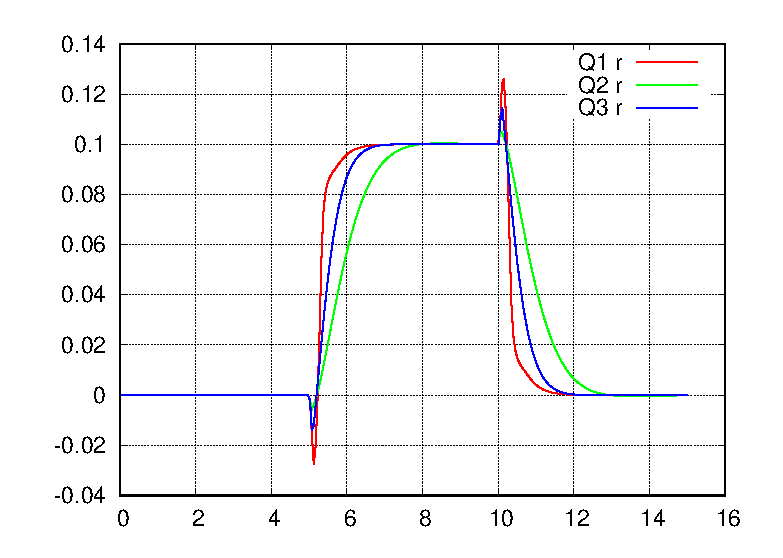
\includegraphics[width=1.0\linewidth]{CompareQ_r.eps}
            \caption{図\ref{sim_Q_r}: 重み行列による比較(台車位置)}
            \label{sim_Q_r}
        \end{center}
    \end{minipage}
    \begin{minipage}{0.5\hsize}
        \begin{center}
            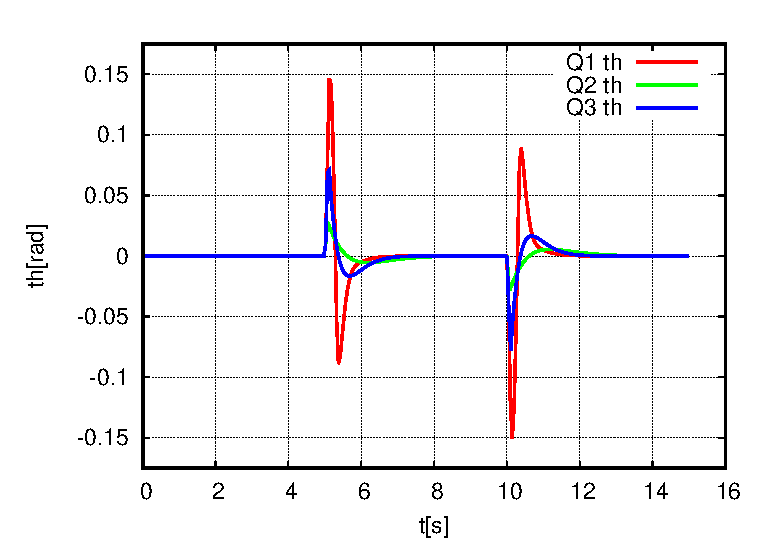
\includegraphics[width=1.0\linewidth]{CompareQ_th.eps}
            \caption{図\ref{sim_Q_th}: 重み行列による比較(振子角度})
            \label{sim_Q_th}
        \end{center}
    \end{minipage}
\end{figure}

図\ref{sim_Q_r}から,最も重みを大きくしたパターン1をみると,たしかに台車の目標位置への収束は速くなっているが,
台車の位置を有線する一方で振子の角度の振幅は大きくなっている.一方で,振子角度の重みを最も大きくしたパターン2では,
振子角度の振幅は小さく抑えられていると同時に,台車位置の目標値への収束が3パターンの中で最も遅くなっている.

\subsection{オブザーバの極変更に関するシミュレーション}
目標値変更における安定化制御で,表\ref{sim_P}に示すパラメータを用いてシミュレーションを行う.

\begin{table}[htbp]
    \begin{center}
        \caption{表\ref{sim_P}: オブザーバの極によるシミュレーションに用いるパラメータの種類}
        \begin{tabular}{|c|c|c|c|c|} \hline
            パターン & 重み行列$Q$ & オブザーバの極$P$ & サンプリング周期$dt$[s] \\ \hline \hline
            パターン1 & $Q_1$(1E6, 1E5, 1, 1) & $P_1$((-23,0), (-23,0)) & $dt_1$:0.005 \\ \hline
            パターン2 & $Q_2$(1E6, 1E5, 1, 1) & $P_2$((-50,0), (-50,0)) & $dt_2$:0.005 \\ \hline
        \end{tabular}
        \label{sim_P}
    \end{center}
\end{table}

表\ref{sim_P}に従ってシミュレーションを行った結果を図\ref{sim_P_r}, 図\ref{sim_P_th}に示す.

\begin{figure}[htbp]
    \begin{minipage}{0.5\hsize}
        \begin{center}
            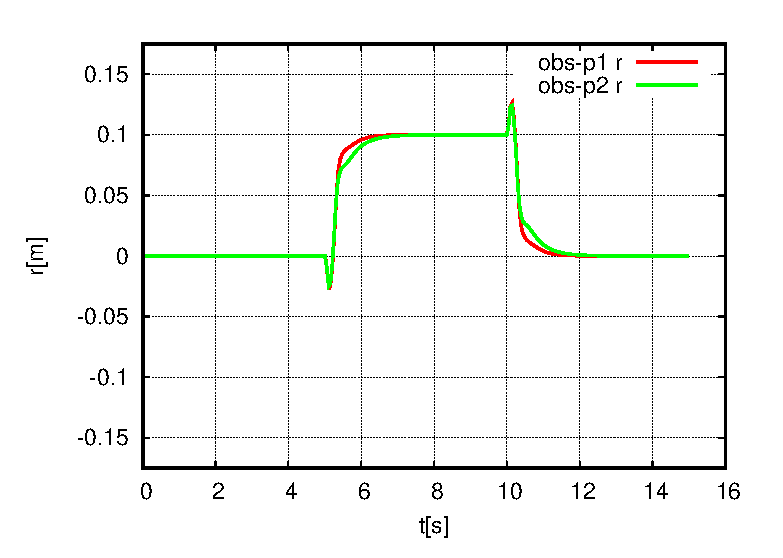
\includegraphics[width=1.0\linewidth]{CompareP_r.eps}
            \caption{図\ref{sim_P_r}: オブザーバの極による比較(台車位置)}
            \label{sim_P_r}
        \end{center}
    \end{minipage}
    \begin{minipage}{0.5\hsize}
        \begin{center}
            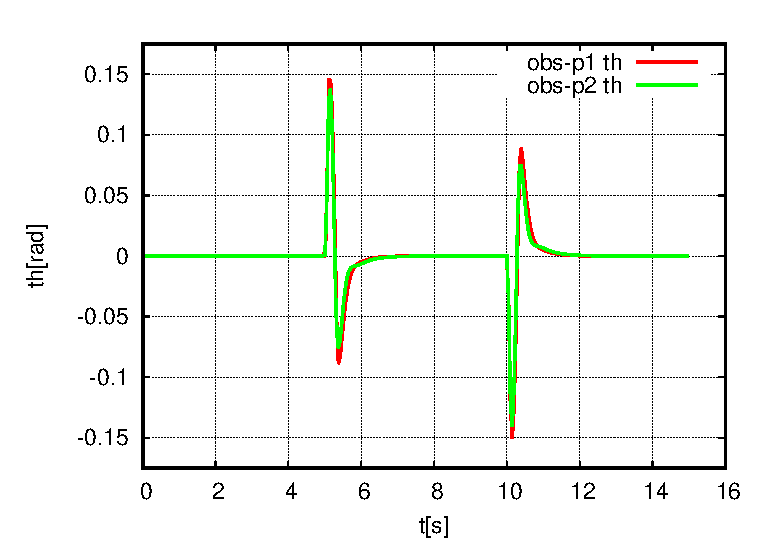
\includegraphics[width=1.0\linewidth]{CompareP_th.eps}
            \caption{図\ref{sim_P_th}: オブザーバの極による比較(振子角度)}
            \label{sim_P_th}
        \end{center}
    \end{minipage}
\end{figure}

台車位置,振子角度だけでは変化が表れにくいので,それぞれのオブザーバの推定誤差を用いて比較を行う.
図\ref{error_obs_r}に台車速度に関する推定誤差を,図\ref{error_obs_th}に振子角速度に関する推定誤差を示す.

\begin{figure}[htbp]
    \begin{minipage}{0.5\hsize}
        \begin{center}
            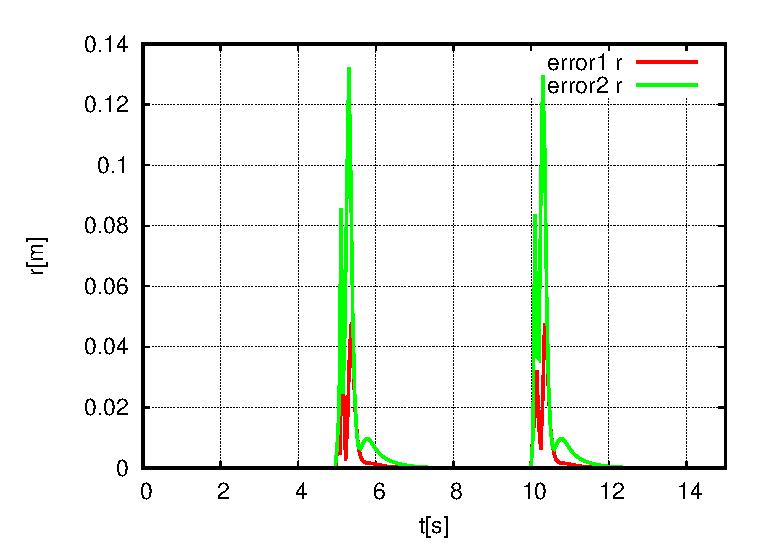
\includegraphics[width=1.0\linewidth]{error_obs_r.eps}
            \caption{図\ref{error_obs_r}: 台車速度の推定誤差}
            \label{error_obs_r}
        \end{center}
    \end{minipage}
    \begin{minipage}{0.5\hsize}
        \begin{center}
            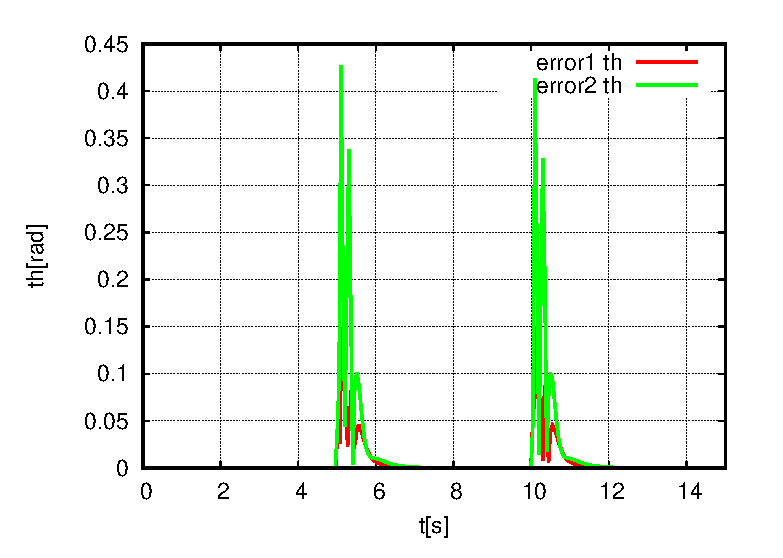
\includegraphics[width=1.0\linewidth]{error_obs_th.eps}
            \caption{図\ref{error_obs_th}: 振子角速度の推定誤差}
            \label{error_obs_th}
        \end{center}
    \end{minipage}
\end{figure}

台車速度,振子角度の推定誤差ともに,オブザーバの極が負の方向に虚軸から遠いほど推定誤差が大きくなっている.
よって,このシミュレーション結果からはオブザーバの極は虚軸に近い極配置が好ましいと言える.
実際には,極の絶対値がより大きいほど推定誤差は小さくなるが,本実験で行ったシミュレーションのパラメータでは
既に極の絶対値が十分に大きく,オブザーバの極配置以外の要因により推定誤差が大きくなったと考察できる.


\subsection{サンプリング周期変更に関するシミュレーション}
目標値変更における安定化制御で,表\ref{sim_Dt}に示すパラメータを用いてシミュレーションを行う.

\begin{table}[htbp]
    \begin{center}
        \caption{表\ref{sim_Dt}: サンプリング周期によるシミュレーションに用いるパラメータの種類}
        \begin{tabular}{|c|c|c|c|c|} \hline
            パターン & 重み行列$Q$ & オブザーバの極$P$ & サンプリング周期$dt$[s] \\ \hline \hline
            パターン1 & $Q_1$(1E6, 1E5, 1, 1) & $P_1$((-23,0), (-23,0)) & $dt_1$:0.005 \\ \hline
            パターン2 & $Q_2$(1E6, 1E5, 1, 1) & $P_2$((-23,0), (-23,0)) & $dt_2$:0.01 \\ \hline
        \end{tabular}
        \label{sim_Dt}
    \end{center}
\end{table}

表\ref{sim_Dt}に従ってシミュレーションを行った結果を図\ref{sim_Dt_r}, 図\ref{sim_Dt_th}に示す.

\begin{figure}[htbp]
    \begin{minipage}{0.5\hsize}
        \begin{center}
            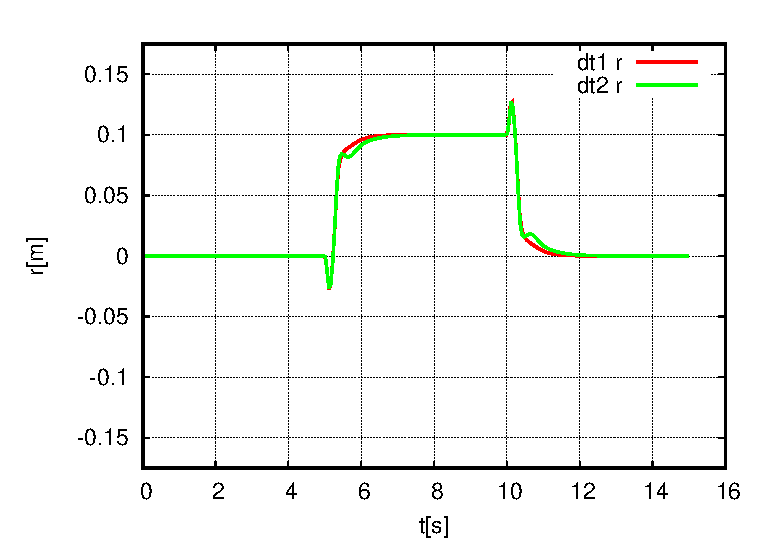
\includegraphics[width=1.0\linewidth]{CompareDt_r.eps}
            \caption{図\ref{sim_Dt_r}: サンプリング周期による比較(台車位置)}
            \label{sim_Dt_r}
        \end{center}
    \end{minipage}
    \begin{minipage}{0.5\hsize}
        \begin{center}
            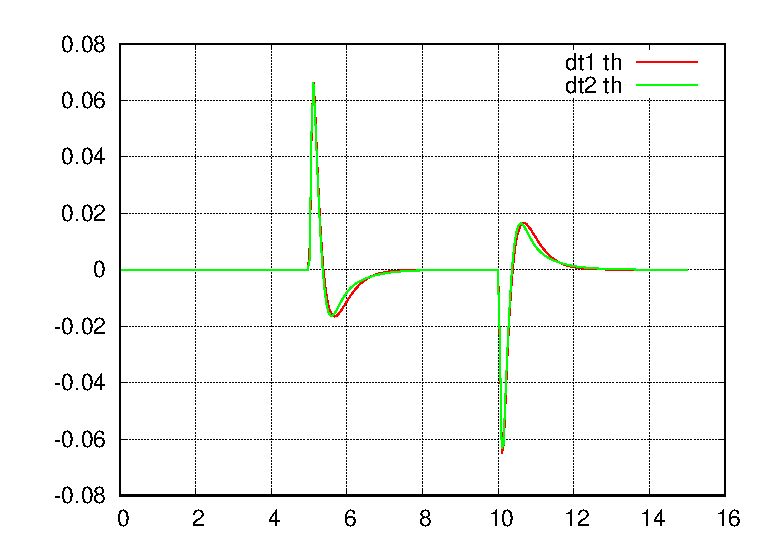
\includegraphics[width=1.0\linewidth]{CompareDt_th.eps}
            \caption{図\ref{sim_Dt_th}: サンプリング周期による比較(振子角度)}
            \label{sim_Dt_th}
        \end{center}
    \end{minipage}
\end{figure}

オブザーバの極によるシミュレーション同様,台車位置,振子角度だけでは変化が表れにくいので,
それぞれのオブザーバの推定誤差を用いて比較を行う.
図\ref{error_dt_r}に台車速度に関する推定誤差を,図\ref{error_dt_th}に振子角速度に関する推定誤差を示す.

\begin{figure}[htbp]
    \begin{minipage}{0.5\hsize}
        \begin{center}
            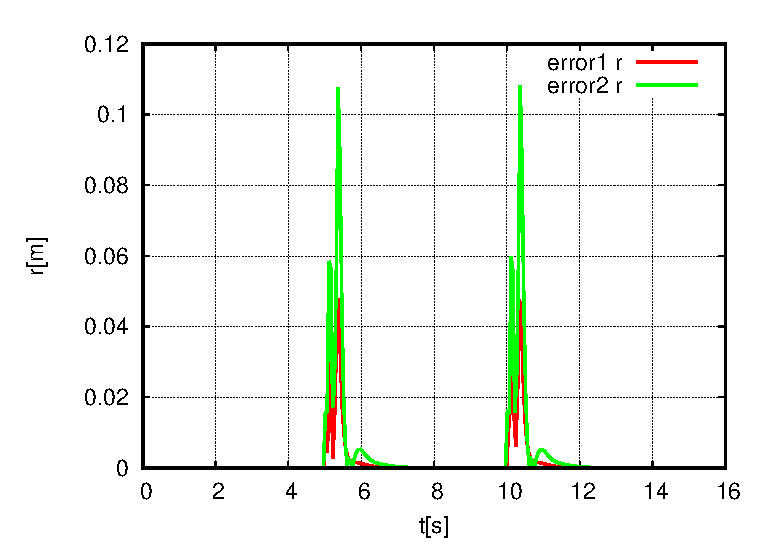
\includegraphics[width=1.0\linewidth]{error_dt_r.eps}
            \caption{図\ref{error_dt_r}: 台車速度の推定誤差}
            \label{error_dt_r}
        \end{center}
    \end{minipage}
    \begin{minipage}{0.5\hsize}
        \begin{center}
            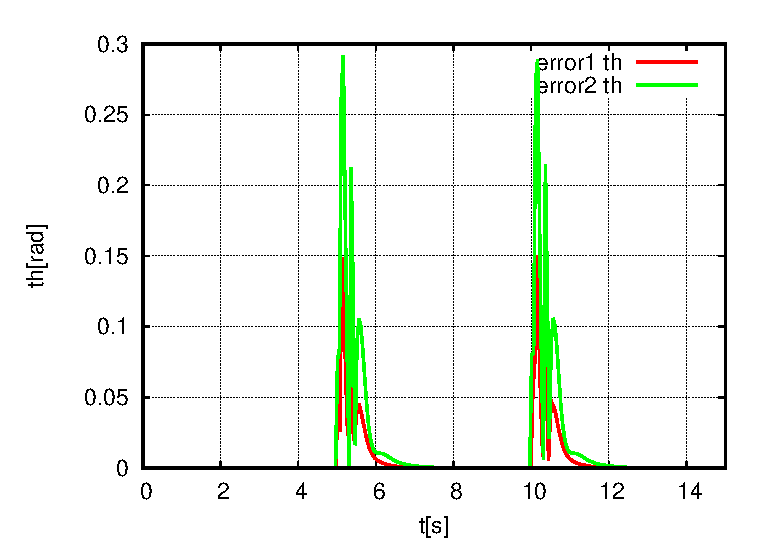
\includegraphics[width=1.0\linewidth]{error_dt_th.eps}
            \caption{図\ref{error_dt_th}: 振子角速度の推定誤差}
            \label{error_dt_th}
        \end{center}
    \end{minipage}
\end{figure}

図\ref{error_dt_r},図\ref{error_dt_th}から,サンプリング周期が短いほど推定誤差が小さくなっている.
サンプリング周期を大きくすると,計測するデータの間隔が大きくなってしまうため,実際の値への追従が遅れる.
よって,このシミュレーションでは意図した結果が得られたと言える.


\subsection{振り上げ制御のシミュレーション}
振り上げシミュレーションに用いたパラメータを表\ref{sim_swing}に示す.
ただし,振子が安定化制御に移行した際に用いるパラメータは表\ref{swing_stable}のパラメータを用いることとする.
また,台車位置,振子角度の制限として,台車位置はベルト中心から両方向に$0.09$[m],振子角度は
$\left[-\pi\right.,\ \left.\pi\right)$[rad]の範囲の値を取るものとする.

\begin{table}[htbp]
    \begin{center}
        \caption{表\ref{sim_swing}: 振り上げ制御のシミュレーションに用いるパラメータの種類}
        \begin{tabular}{|c|c|c|} \hline
            パターン & $k$ & $n$ \\ \hline \hline
            パターン1 & $1.0\mbox{E}3$ & $0.31$ \\ \hline
            パターン2 & $1.0\mbox{E}4$ & $0.31$ \\ \hline
            パターン3 & $1.0\mbox{E}5$ & $0.31$ \\ \hline
        \end{tabular}
        \label{sim_swing}
    \end{center}
\end{table}

\begin{table}[htbp]
    \begin{center}
        \caption{表\ref{swing_stable}: 振り上げ後の安定化制御に用いるパラメータ}
        \begin{tabular}{|c|c|c|c|} \hline
            重み行列$Q$ & オブザーバの極$P$ & サンプリング周期$dt$[s] \\ \hline \hline
            $Q$(1E6, 1E5, 1, 1) & $P$((-23,0), (-23,0)) & $dt$:0.005 \\ \hline
          \end{tabular}
        \label{swing_stable}
    \end{center}
\end{table}

表\ref{sim_swing}を用いて振り上げ制御のシミュレーションを行った結果を図\ref{sim_swing_r},
図\ref{sim_swing_th}に示す.

\begin{figure}[htbp]
    \begin{minipage}{0.5\hsize}
        \begin{center}
            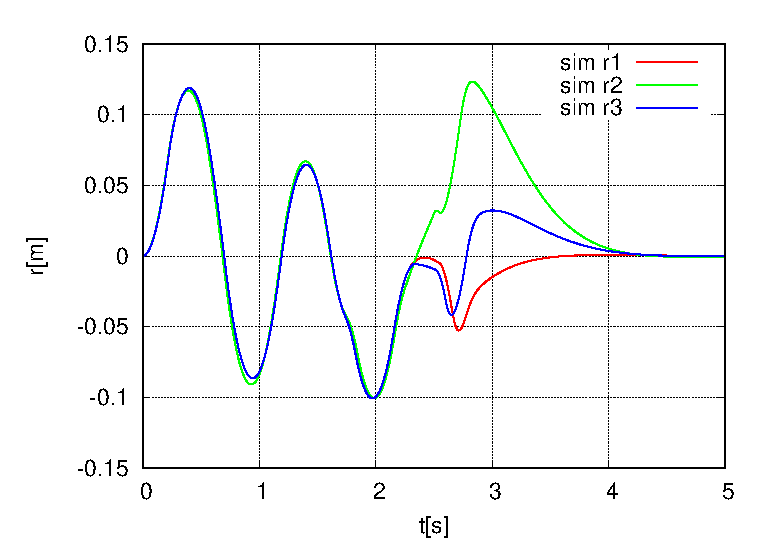
\includegraphics[width=1.0\linewidth]{swing_sim_r.eps}
            \caption{図\ref{sim_swing_r}: 台車位置}
            \label{sim_swing_r}
        \end{center}
    \end{minipage}
    \begin{minipage}{0.5\hsize}
        \begin{center}
            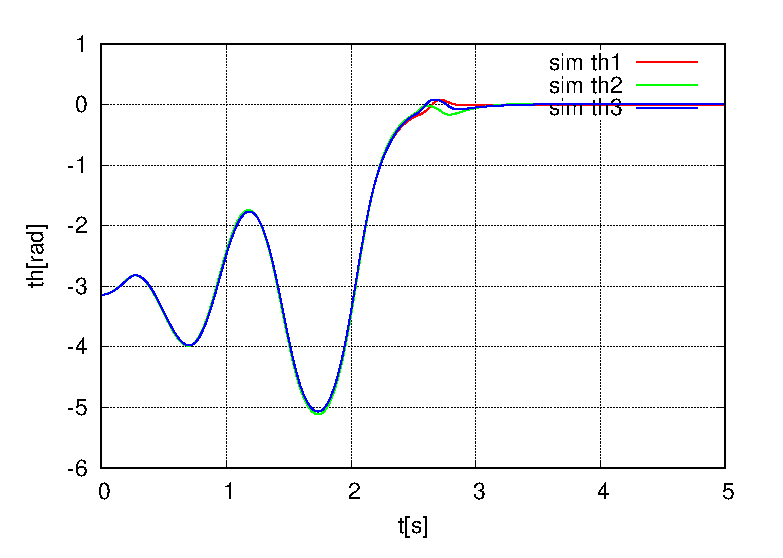
\includegraphics[width=1.0\linewidth]{swing_sim_th.eps}
            \caption{図\ref{sim_swing_th}: 振子角度}
            \label{sim_swing_th}
        \end{center}
    \end{minipage}
\end{figure}

パラメータ$k$の値を大きくすることで,目標とする振子の運動エネルギーへの収束が速くなることが予想されたが,
本実験のシミュレーションでは$k$の値に関わらず安定化制御に移行するまでの時間に変化はなかった.
ただし,安定化制御に移行する際の台車位置はそれぞれ異なっていたため,パラメータ$k$の値によっては
台車が制限された移動範囲外にはみ出してしまう可能性がある.

% =============================== chapter 4 END =============================== %

% --- Chapter 4 END --- %

% ----- chapter 5 ----- %
% ================================= chapter 5 ================================= %
\chapter{実験}

\subsection{実験装置}
本実験で用いる実験装置を図\ref{my_pend}に示す.この実験装置は第\ref{chapter_modeling}章で示した実験装置と
同様の機能を有する.

\begin{figure}[htbp]
    \begin{center}
        \includegraphics[width=0.6\linewidth]{my_pend.eps}
        \caption{図\ref{my_pend}: 本実験で使用した倒立振子}
        \label{my_pend}
    \end{center}
\end{figure}


\subsection{安定化制御の実験}
表\ref{sim_Q}から表\ref{sim_Dt}までのパラメータを用いて,目標値変更における安定化制御を行う.
振子が鉛直上向きの状態から安定化制御を開始し,$5$秒ごとに台車の目標値を
$0.0 \to 0.5 \to 0.0$[m]と交互に切り替える.

\subsection{重み行列}
重み行列の変化による実験結果を図\ref{exp_Q_r},図\ref{exp_Q_th}に示す.

\begin{figure}[htbp]
    \begin{minipage}{0.5\hsize}
        \begin{center}
            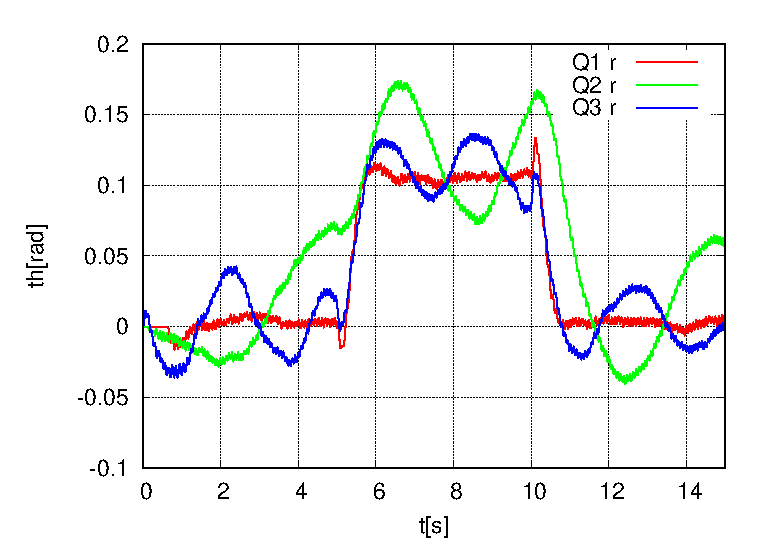
\includegraphics[width=1.0\linewidth]{case3_5_11_r.eps}
            \caption{図\ref{exp_Q_r}: 重み行列による比較(台車位置)}
            \label{exp_Q_r}
        \end{center}
    \end{minipage}
    \begin{minipage}{0.5\hsize}
        \begin{center}
            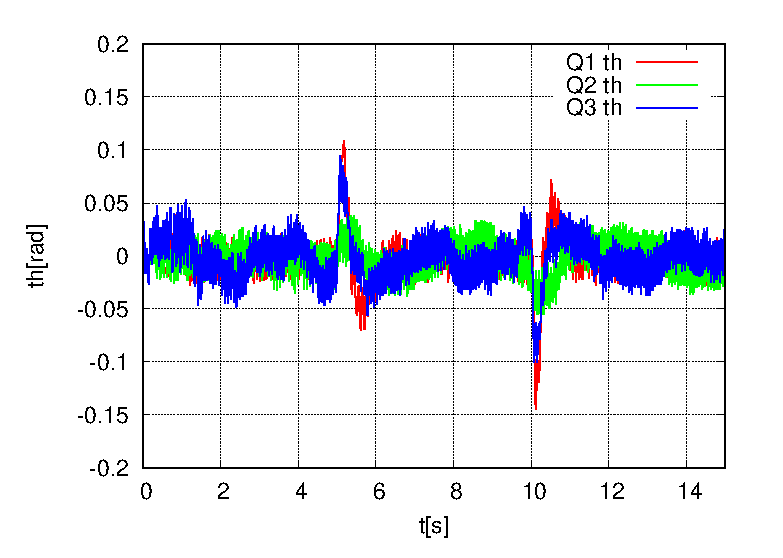
\includegraphics[width=1.0\linewidth]{case3_5_11_th.eps}
            \caption{図\ref{exp_Q_th}: 重み行列による比較(振子角度})
            \label{exp_Q_th}
        \end{center}
    \end{minipage}
\end{figure}

台車位置の重みを最も大きくしたパターン1の波形に着目すると,3パターンの中で最も速く台車位置が目標値に収束している.
一方,振子角度の重みを最も大きくしたパターン2の台車位置は,目標値に収束する前に目標値が変更され,常に振動的な
応答となっている.振子角度についてもシミュレーションの場合と同様のことが言える.


\subsection{オブザーバの極}
オブザーバの極の変化に関する実験結果を図\ref{exp_P_r},図\ref{exp_P_th}に示す.

\begin{figure}[htbp]
    \begin{minipage}{0.5\hsize}
        \begin{center}
            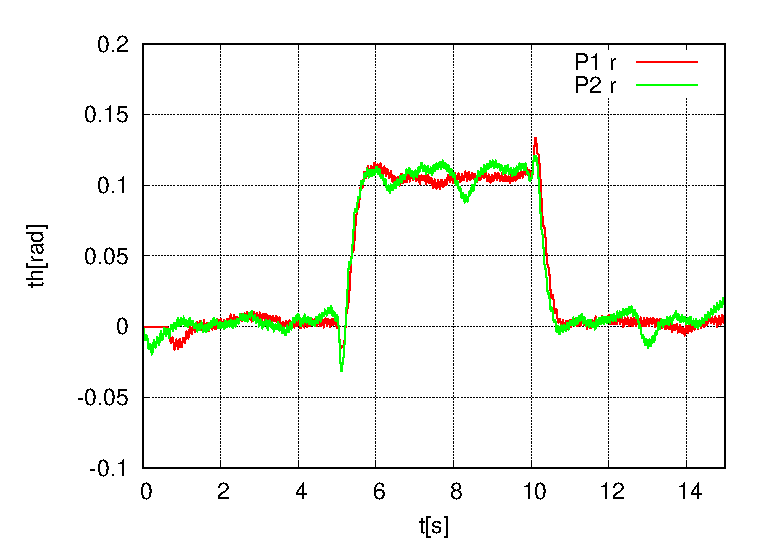
\includegraphics[width=1.0\linewidth]{case3_4_r.eps}
            \caption{図\ref{exp_P_r}: オブザーバの極による比較(台車位置)}
            \label{exp_P_r}
        \end{center}
    \end{minipage}
    \begin{minipage}{0.5\hsize}
        \begin{center}
            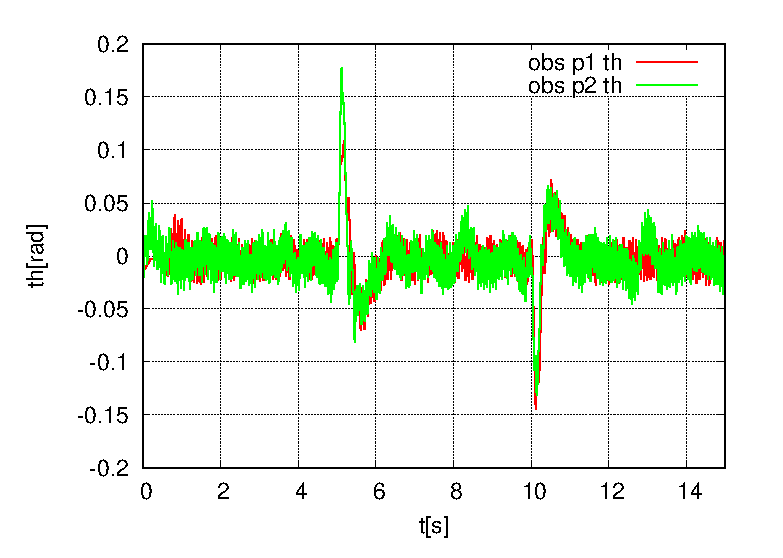
\includegraphics[width=1.0\linewidth]{case3_4_th.eps}
            \caption{図\ref{exp_P_th}: オブザーバの極による比較(振子角度)}
            \label{exp_P_th}
        \end{center}
    \end{minipage}
\end{figure}

シミュレーションの場合と同様,台車位置と振子角度に大きな変化は見られなかった.


\subsection{サンプリング周期}
サンプリング周期の変化に関する実験結果を図\ref{exp_Dt_r},図\ref{exp_Dt_th}に示す.

\begin{figure}[htbp]
    \begin{minipage}{0.5\hsize}
        \begin{center}
            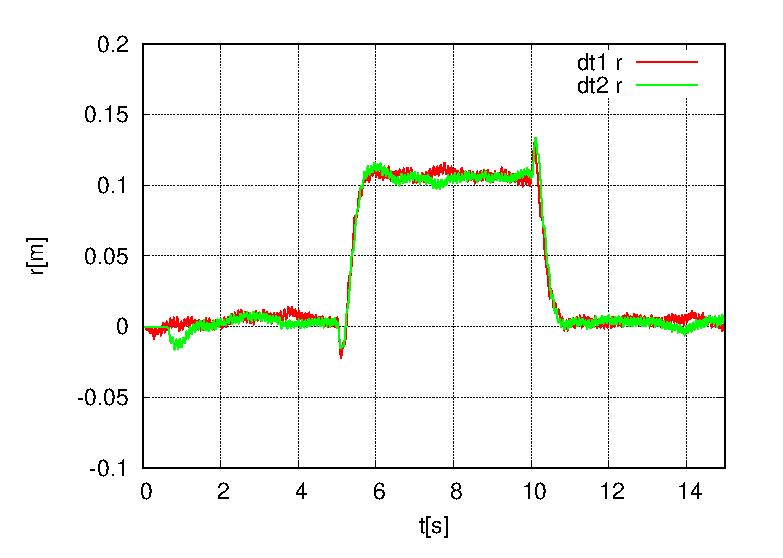
\includegraphics[width=1.0\linewidth]{case1_3_r.eps}
            \caption{図\ref{exp_Dt_r}: サンプリング周期による比較(台車位置)}
            \label{exp_Dt_r}
        \end{center}
    \end{minipage}
    \begin{minipage}{0.5\hsize}
        \begin{center}
            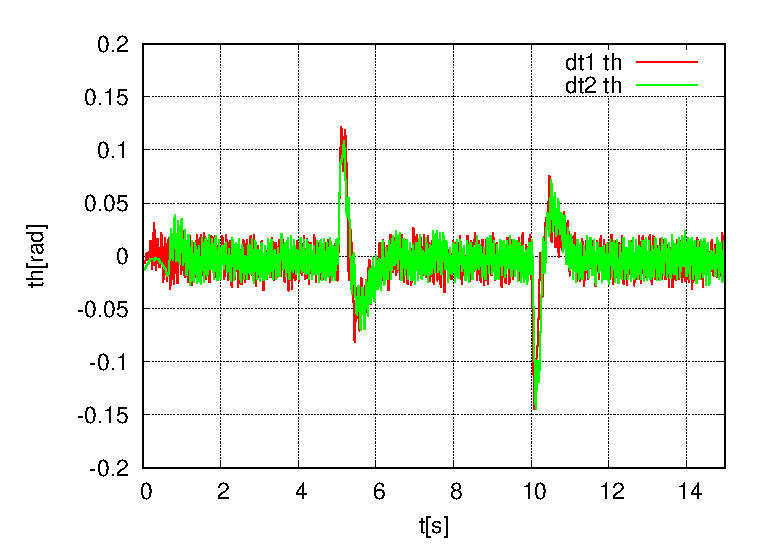
\includegraphics[width=1.0\linewidth]{case1_3_th.eps}
            \caption{図\ref{exp_Dt_th}: サンプリング周期による比較(振子角度)}
            \label{exp_Dt_th}
        \end{center}
    \end{minipage}
\end{figure}

シミュレーションの場合と同様,台車位置と振子角度に大きな変化は見られなかった.


\subsection{シミュレーションと実験結果の比較}
表\ref{sim_exp}をもとに,シミュレーションと実験結果を比較した図を,図\ref{case01_r}から図\ref{case12_th}に示す.

\begin{table}[htbp]
	\begin{center}
    \caption{表\ref{sim_exp}: シミュレーションと実験の比較に用いるパラメータ}
		\begin{tabular}{|c|c|c|c|} \hline
			パターン & 重み行列$Q$ & オブザーバの極$P$ & サンプリング周期$dt$ \\ \hline\hline
			パターン01 & diag(1.0E6, 1.0E5, 1, 1) & (-23, -23) & 0.01  \\ \hline
			パターン02 & diag(1.0E6, 1.0E5, 1, 1) & (-50, -50) & 0.01  \\ \hline
			パターン03 & diag(1.0E6, 1.0E5, 1, 1) & (-23, -23) & 0.005 \\ \hline
			パターン04 & diag(1.0E6, 1.0E5, 1, 1) & (-50, -50) & 0.005 \\ \hline
			パターン05 & diag(1.0E5, 1.0E6, 1, 1) & (-23, -23) & 0.005 \\ \hline
			パターン06 & diag(1.0E5, 1.0E6, 1, 1) & (-50, -50) & 0.005 \\ \hline
			パターン07 & diag(1.0E5, 1.0E6, 1, 1) & (-23, -23) & 0.01  \\ \hline
			パターン08 & diag(1.0E5, 1.0E6, 1, 1) & (-50, -50) & 0.01  \\ \hline
			パターン09 & diag(1.0E6, 1.0E6, 1, 1) & (-23, -23) & 0.01  \\ \hline
			パターン10 & diag(1.0E6, 1.0E6, 1, 1) & (-50, -50) & 0.01  \\ \hline
			パターン11 & diag(1.0E6, 1.0E6, 1, 1) & (-23, -23) & 0.005 \\ \hline
			パターン12 & diag(1.0E6, 1.0E6, 1, 1) & (-50, -50) & 0.005 \\ \hline
		\end{tabular}
		\label{sim_exp}
	\end{center}
\end{table}

% --- patter 01 --- %
\begin{figure}[htbp]
    \begin{minipage}{0.5\hsize}
        \begin{center}
            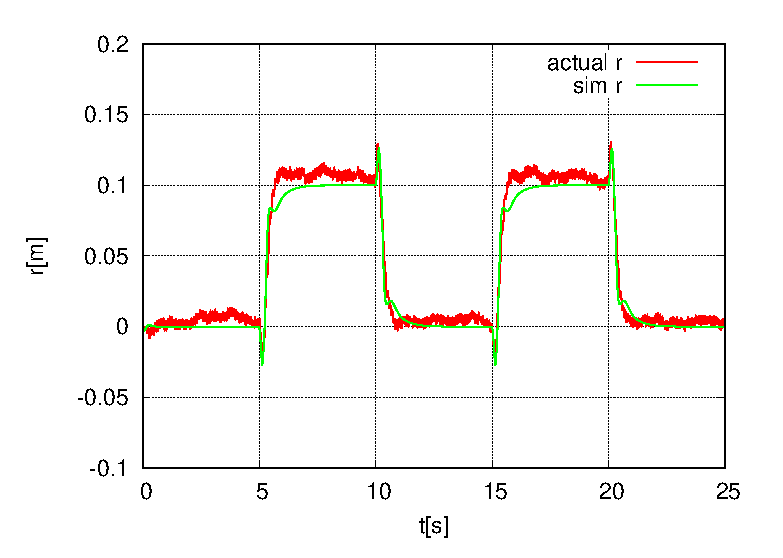
\includegraphics[width=1.0\linewidth]{case1_r.eps}
            \caption{図\ref{case01_r}: パターン01の台車位置}
            \label{case01_r}
        \end{center}
    \end{minipage}
    \begin{minipage}{0.5\hsize}
        \begin{center}
            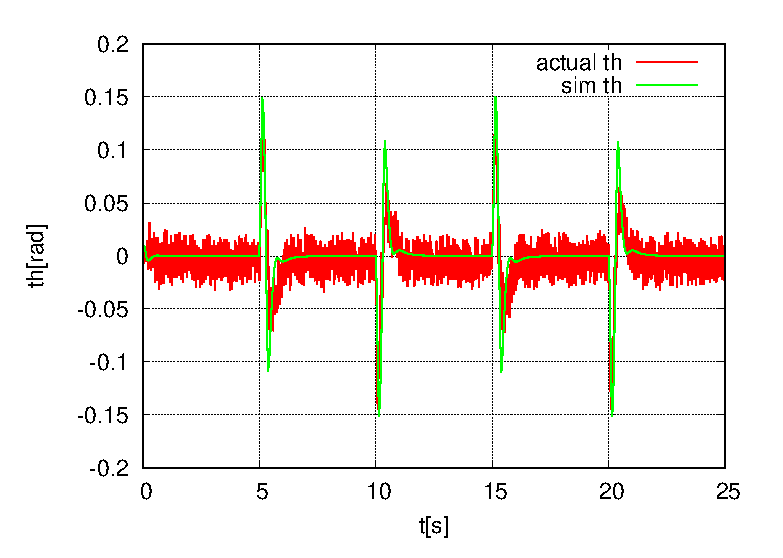
\includegraphics[width=1.0\linewidth]{case1_th.eps}
            \caption{図\ref{case01_th}: パターン01の振子角度}
            \label{case01_th}
        \end{center}
    \end{minipage}
\end{figure}

% --- patter 02 --- %
\begin{figure}[htbp]
    \begin{minipage}{0.5\hsize}
        \begin{center}
            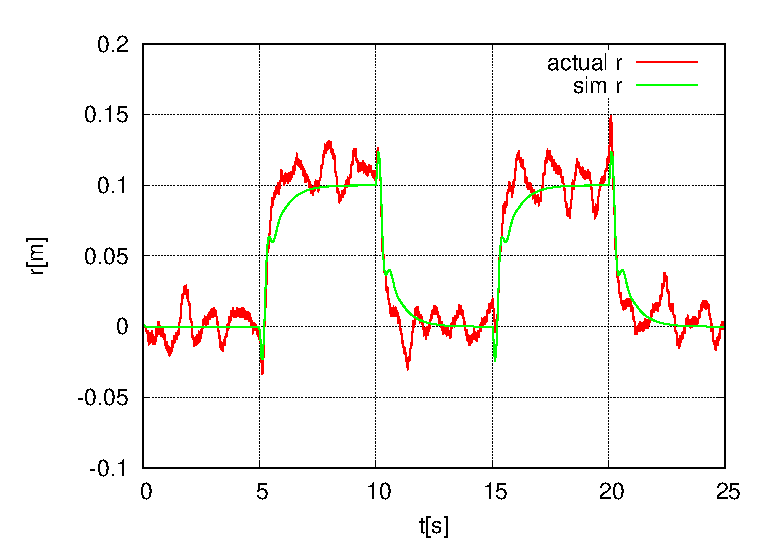
\includegraphics[width=1.0\linewidth]{case2_r.eps}
            \caption{図\ref{case02_r}: パターン02の台車位置}
            \label{case02_r}
        \end{center}
    \end{minipage}
    \begin{minipage}{0.5\hsize}
        \begin{center}
            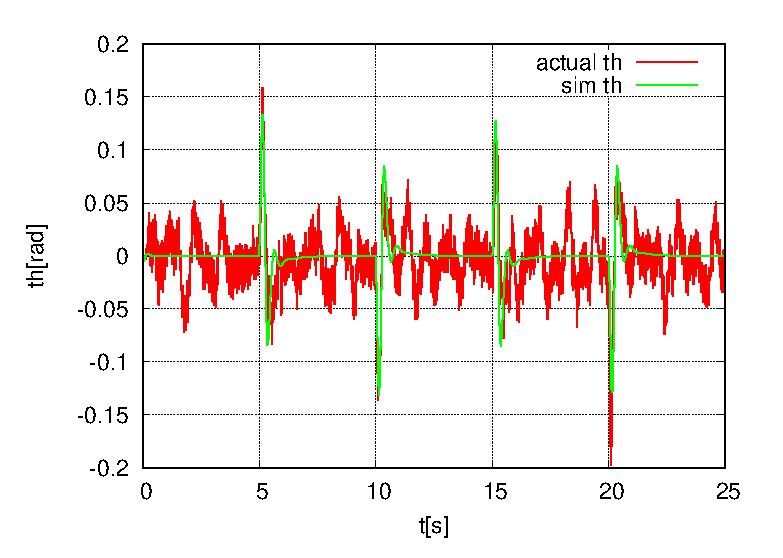
\includegraphics[width=1.0\linewidth]{case2_th.eps}
            \caption{図\ref{case02_th}: パターン02の振子角度}
            \label{case02_th}
        \end{center}
    \end{minipage}
\end{figure}

% --- patter 03 --- %
\begin{figure}[htbp]
    \begin{minipage}{0.5\hsize}
        \begin{center}
            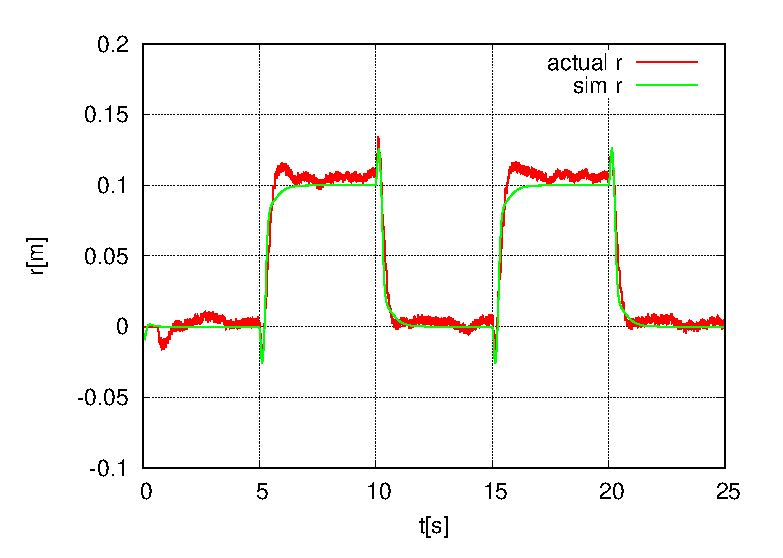
\includegraphics[width=1.0\linewidth]{case3_r.eps}
            \caption{図\ref{case03_r}: パターン03の台車位置}
            \label{case03_r}
        \end{center}
    \end{minipage}
    \begin{minipage}{0.5\hsize}
        \begin{center}
            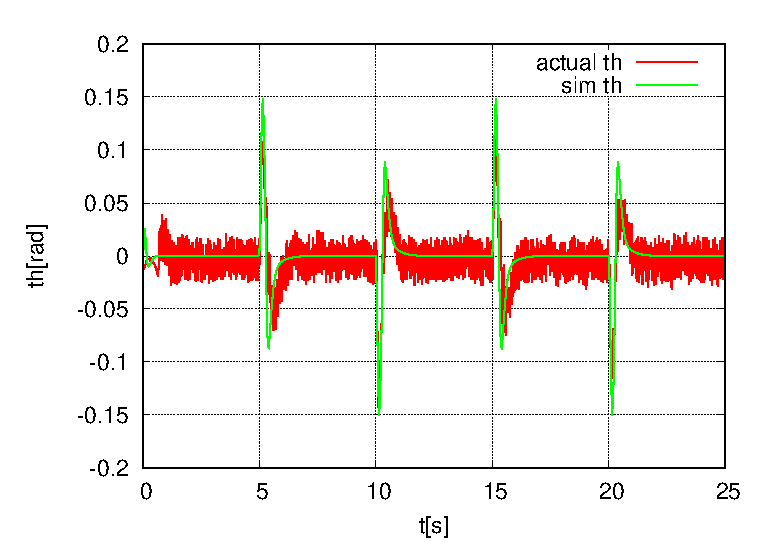
\includegraphics[width=1.0\linewidth]{case3_th.eps}
            \caption{図\ref{case03_th}: パターン03の振子角度}
            \label{case03_th}
        \end{center}
    \end{minipage}
\end{figure}

% --- patter 04 --- %
\begin{figure}[htbp]
    \begin{minipage}{0.5\hsize}
        \begin{center}
            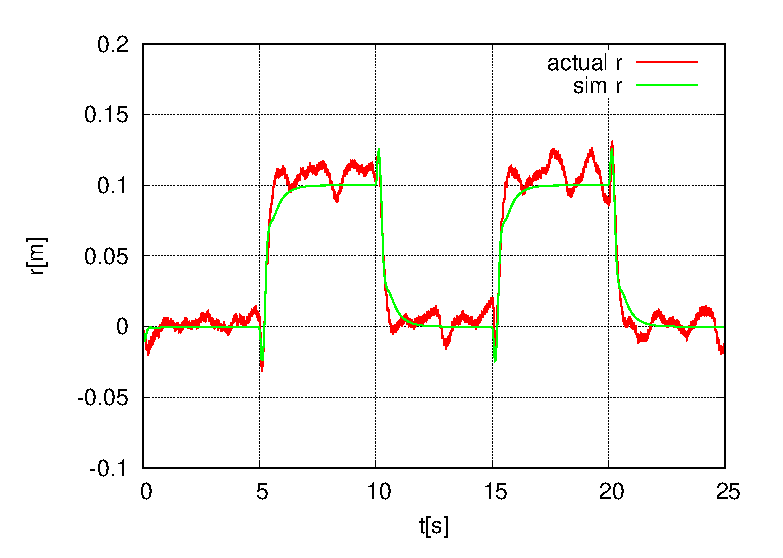
\includegraphics[width=1.0\linewidth]{case4_r.eps}
            \caption{図\ref{case04_r}: パターン04の台車位置}
            \label{case04_r}
        \end{center}
    \end{minipage}
    \begin{minipage}{0.5\hsize}
        \begin{center}
            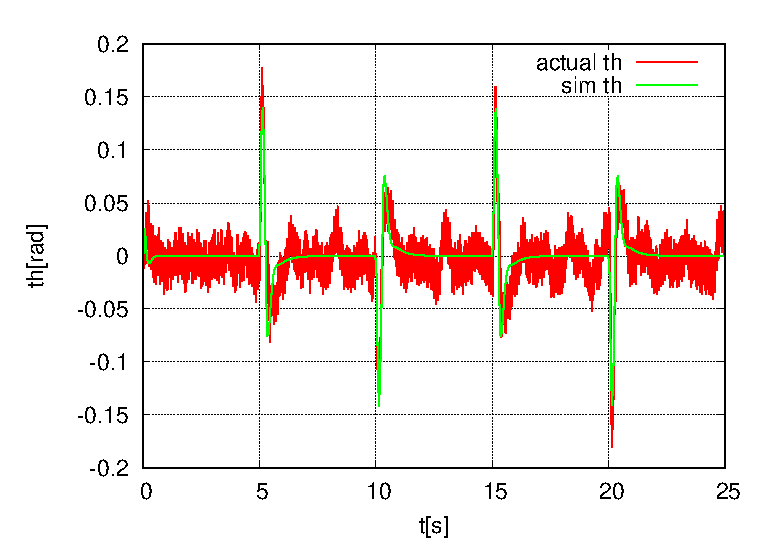
\includegraphics[width=1.0\linewidth]{case4_th.eps}
            \caption{図\ref{case04_th}: パターン04の振子角度}
            \label{case04_th}
        \end{center}
    \end{minipage}
\end{figure}

% --- patter 05 --- %
\begin{figure}[htbp]
    \begin{minipage}{0.5\hsize}
        \begin{center}
            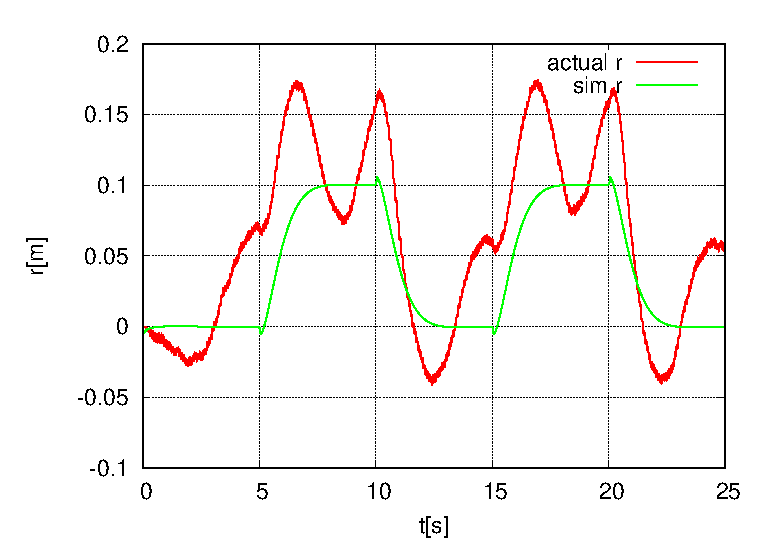
\includegraphics[width=1.0\linewidth]{case5_r.eps}
            \caption{図\ref{case05_r}: パターン05の台車位置}
            \label{case05_r}
        \end{center}
    \end{minipage}
    \begin{minipage}{0.5\hsize}
        \begin{center}
            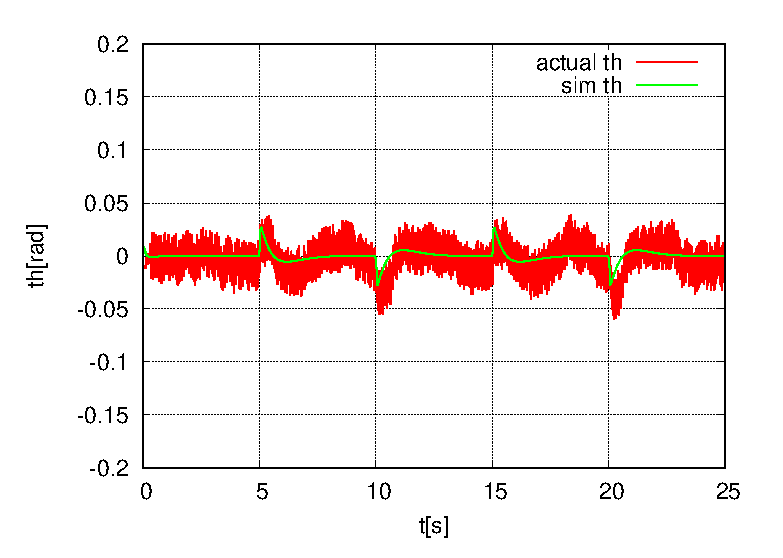
\includegraphics[width=1.0\linewidth]{case5_th.eps}
            \caption{図\ref{case05_th}: パターン05の振子角度}
            \label{case05_th}
        \end{center}
    \end{minipage}
\end{figure}

% --- patter 06 --- %
\begin{figure}[htbp]
    \begin{minipage}{0.5\hsize}
        \begin{center}
            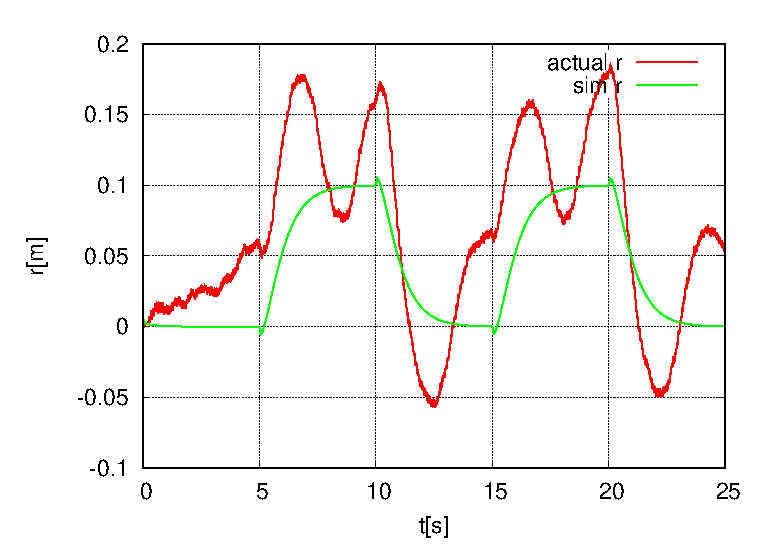
\includegraphics[width=1.0\linewidth]{case6_r.eps}
            \caption{図\ref{case06_r}: パターン06の台車位置}
            \label{case06_r}
        \end{center}
    \end{minipage}
    \begin{minipage}{0.5\hsize}
        \begin{center}
            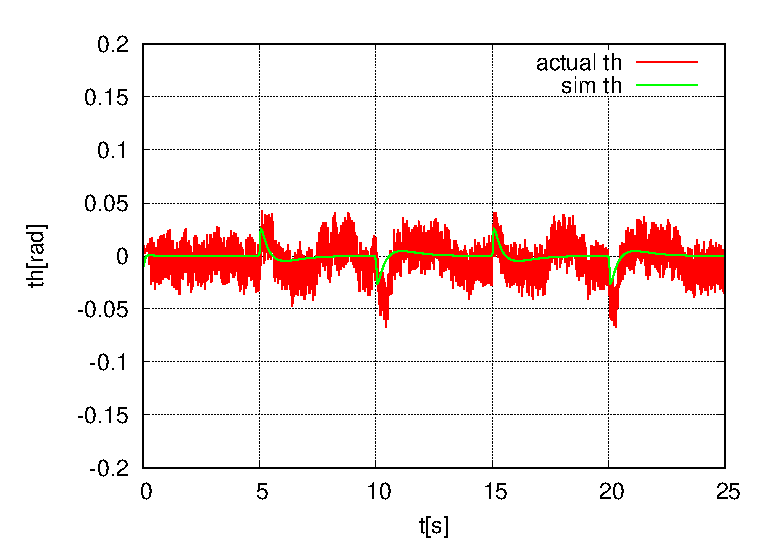
\includegraphics[width=1.0\linewidth]{case6_th.eps}
            \caption{図\ref{case06_th}: パターン06の振子角度}
            \label{case06_th}
        \end{center}
    \end{minipage}
\end{figure}

% --- patter 07 --- %
\begin{figure}[htbp]
    \begin{minipage}{0.5\hsize}
        \begin{center}
            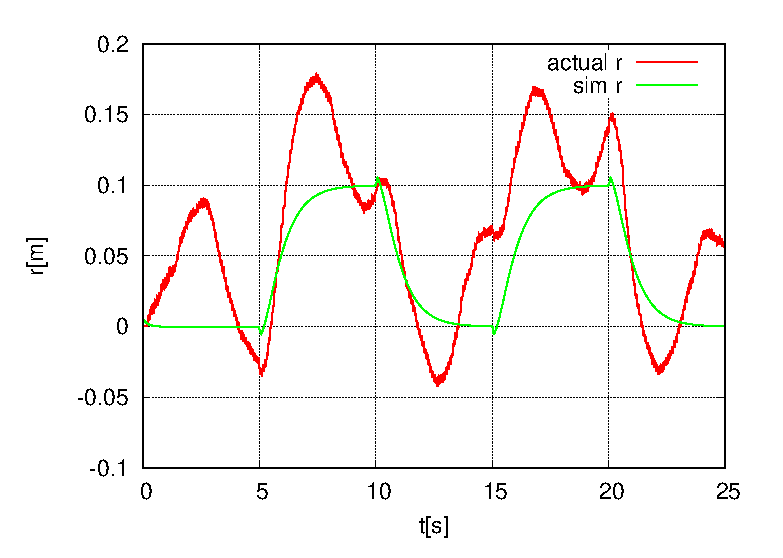
\includegraphics[width=1.0\linewidth]{case7_r.eps}
            \caption{図\ref{case07_r}: パターン07の台車位置}
            \label{case07_r}
        \end{center}
    \end{minipage}
    \begin{minipage}{0.5\hsize}
        \begin{center}
            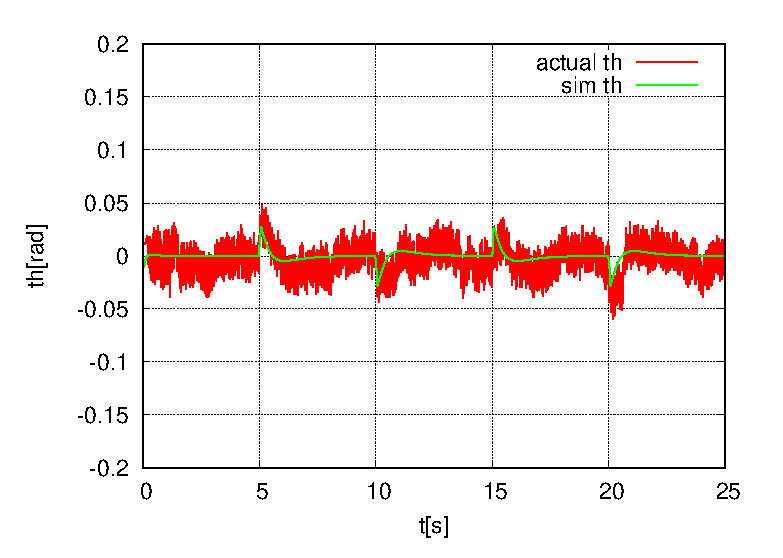
\includegraphics[width=1.0\linewidth]{case7_th.eps}
            \caption{図\ref{case07_th}: パターン07の振子角度}
            \label{case07_th}
        \end{center}
    \end{minipage}
\end{figure}

% --- patter 08 --- %
\begin{figure}[htbp]
    \begin{minipage}{0.5\hsize}
        \begin{center}
            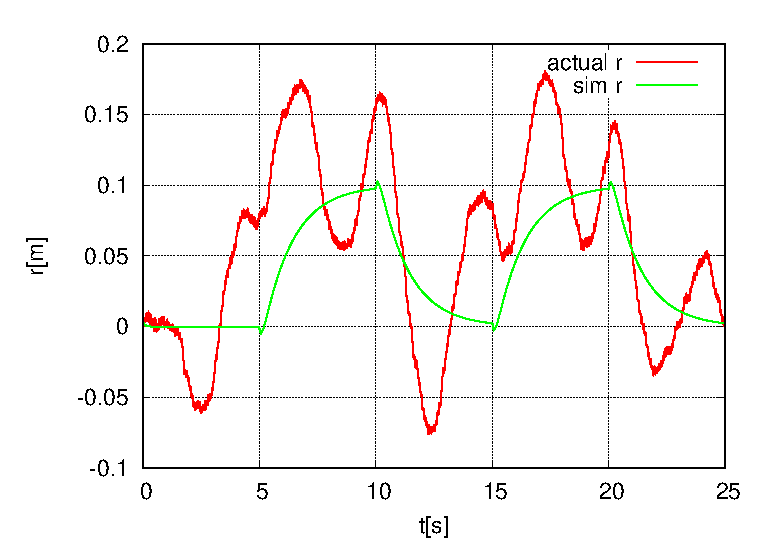
\includegraphics[width=1.0\linewidth]{case8_r.eps}
            \caption{図\ref{case08_r}: パターン08の台車位置}
            \label{case08_r}
        \end{center}
    \end{minipage}
    \begin{minipage}{0.5\hsize}
        \begin{center}
            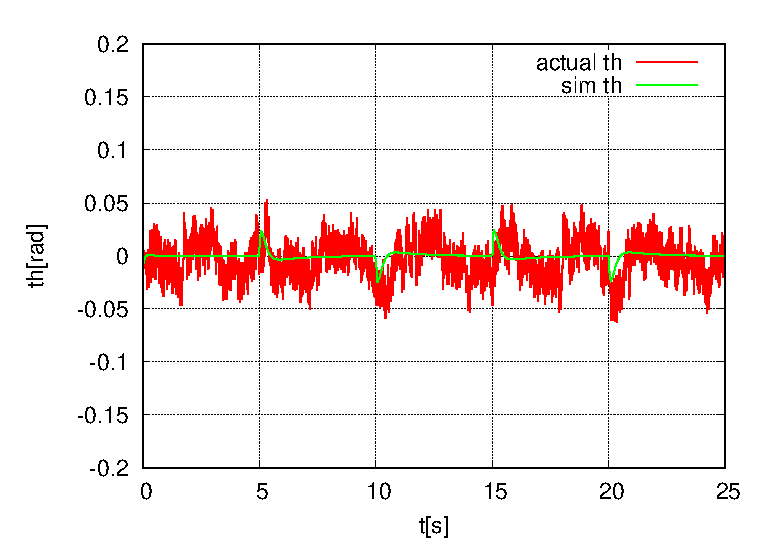
\includegraphics[width=1.0\linewidth]{case8_th.eps}
            \caption{図\ref{case08_th}: パターン08の振子角度}
            \label{case08_th}
        \end{center}
    \end{minipage}
\end{figure}

% --- patter 09 --- %
\begin{figure}[htbp]
    \begin{minipage}{0.5\hsize}
        \begin{center}
            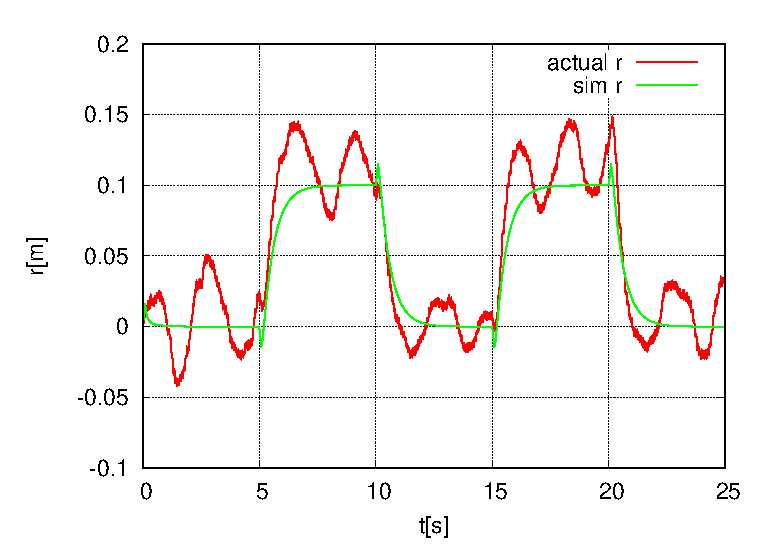
\includegraphics[width=1.0\linewidth]{case9_r.eps}
            \caption{図\ref{case09_r}: パターン09の台車位置}
            \label{case09_r}
        \end{center}
    \end{minipage}
    \begin{minipage}{0.5\hsize}
        \begin{center}
            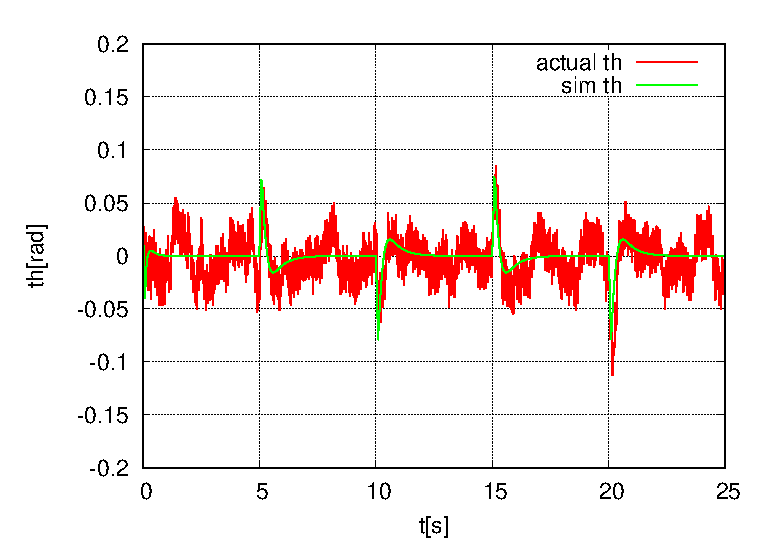
\includegraphics[width=1.0\linewidth]{case9_th.eps}
            \caption{図\ref{case09_th}: パターン09の振子角度}
            \label{case09_th}
        \end{center}
    \end{minipage}
\end{figure}

% --- patter 10 --- %
\begin{figure}[htbp]
    \begin{minipage}{0.5\hsize}
        \begin{center}
            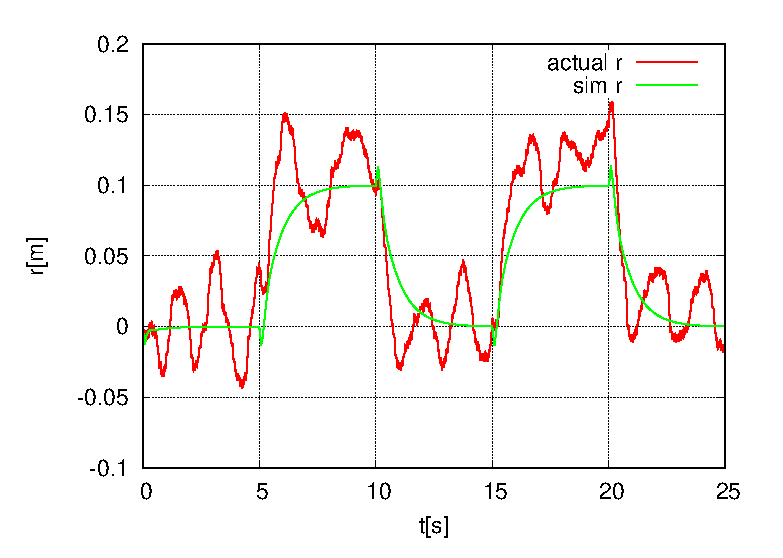
\includegraphics[width=1.0\linewidth]{case10_r.eps}
            \caption{図\ref{case10_r}: パターン10の台車位置}
            \label{case10_r}
        \end{center}
    \end{minipage}
    \begin{minipage}{0.5\hsize}
        \begin{center}
            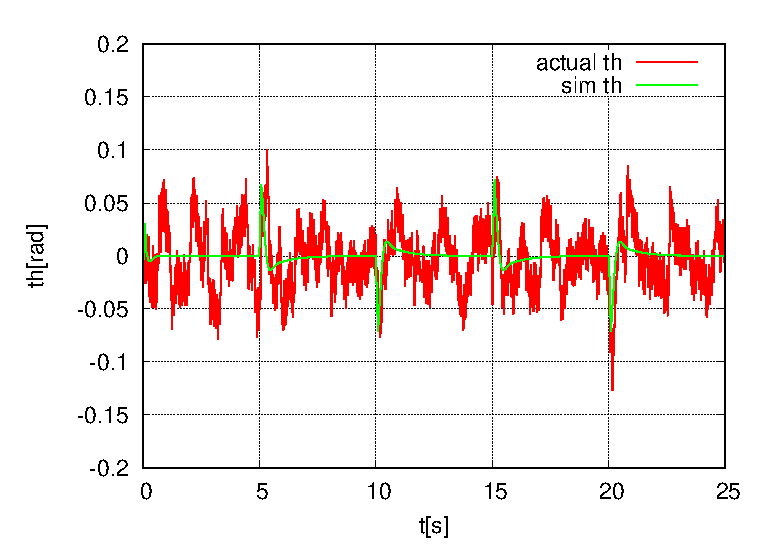
\includegraphics[width=1.0\linewidth]{case10_th.eps}
            \caption{図\ref{case10_th}: パターン10の振子角度}
            \label{case10_th}
        \end{center}
    \end{minipage}
\end{figure}

% --- patter 11 --- %
\begin{figure}[htbp]
    \begin{minipage}{0.5\hsize}
        \begin{center}
            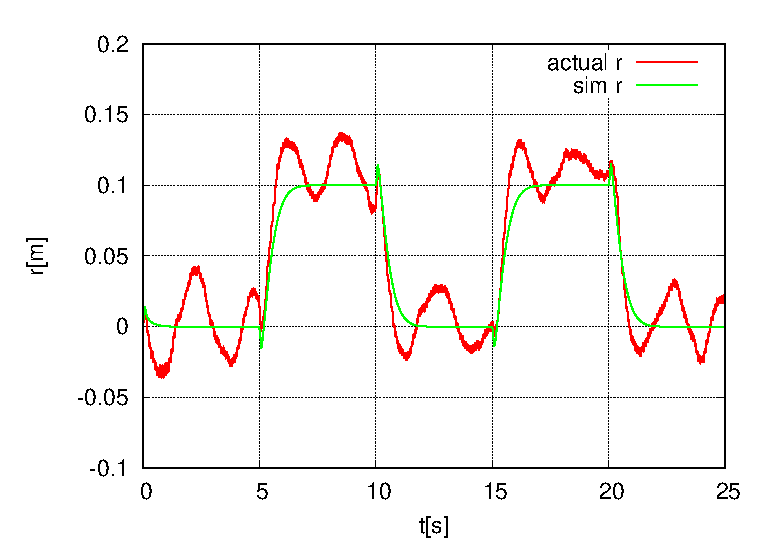
\includegraphics[width=1.0\linewidth]{case11_r.eps}
            \caption{図\ref{case11_r}: パターン11の台車位置}
            \label{case11_r}
        \end{center}
    \end{minipage}
    \begin{minipage}{0.5\hsize}
        \begin{center}
            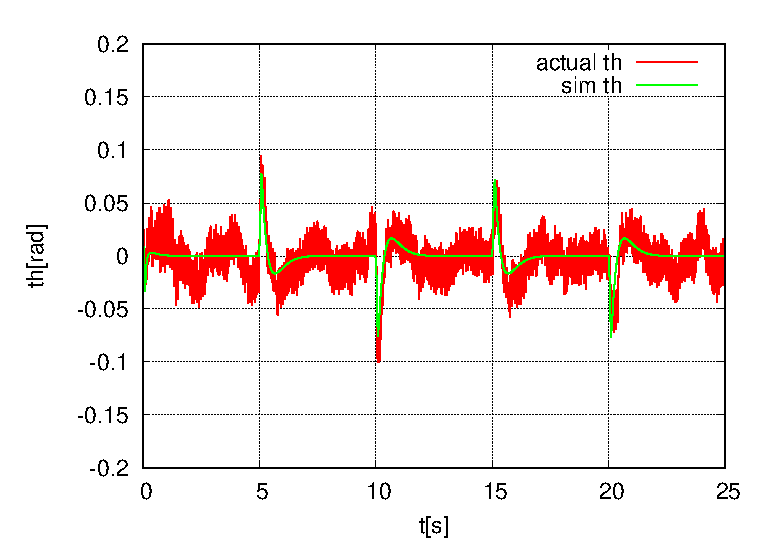
\includegraphics[width=1.0\linewidth]{case11_th.eps}
            \caption{図\ref{case11_th}: パターン11の振子角度}
            \label{case11_th}
        \end{center}
    \end{minipage}
\end{figure}

% --- patter 12 --- %
\begin{figure}[htbp]
    \begin{minipage}{0.5\hsize}
        \begin{center}
            \includegraphics[width=1.0\linewidth]{case12_r.eps}
            \caption{図\ref{case12_r}: パターン12の台車位置}
            \label{case12_r}
        \end{center}
    \end{minipage}
    \begin{minipage}{0.5\hsize}
        \begin{center}
            \includegraphics[width=1.0\linewidth]{case12_th.eps}
            \caption{図\ref{case12_th}: パターン12の振子角度}
            \label{case12_th}
        \end{center}
    \end{minipage}
\end{figure}

\subsection{目標値変更における安定化制御に関する考察}
\begin{itemize}
    \item 重み行列 \\
        振子角度よりも台車位置に重みを置いたパターン01からパターン03と,振子角度と台車位置に同等の
        重みを置いたパターン09からパターン12までを比較すると,台車位置に重みを置いた方が目標値への収束が
        早いことがわかる.逆に,振子角度に重みを置いたパターン03とパターン05では,パターン05の方が
        振子角度の振動が抑えられていることがわかる.
        よって,重み行列の各成分に対応した変位の応答を制御することができた.
    \item オブザーバ \\
        図\ref{case01_r}と図\ref{case02_r}を比較すると,オブザーバの極の実部が実軸負の方向に
        原点から離れているほうが,目標値への収束が早いと考えられる.しかし,今回行った実験の結果では,
        目標値への収束の速さに差異はなく,推定誤差も極が虚軸から遠いほど大きくなっていた.
        シミュレーション,実験で用いたオブザーバの極はすべて十分に大きく,オブザーバ以外の要因によって
        推定誤差,収束速度に変化が表れたと考えられる.
    \item サンプリング周期 \\
        サンプリング周期が小さいほど,短い間隔で状態のフィードバックをかけることができるため,
        より正確なシミュレーション,実験を行うことができる.すなわち,目標値への収束も早くなると言える.
        図\ref{case02_th}, 図\ref{case04_th}を比較すると,サンプリング周期が小さい図\ref{case04_th}
        の方が振動が抑えられ目標値へ早く収束しているため,理論通りの結果が得られたと言える.
\end{itemize}


\subsection{振り上げ制御}
振り上げ制御の実験には,表\ref{sim_swing}のパラメータを用いる.ただし,振子が十分に振り上がり,
安定化制御に移行した後に用いるパラメータは表\ref{swing_stable}の値を用いる.
以上のパラメータを用いた振り上げ制御の実験結果を図\ref{exp_swing_r},図\ref{exp_swing_th}に示す.

\begin{figure}[htbp]
    \begin{minipage}{0.5\hsize}
        \begin{center}
            \includegraphics[width=1.0\linewidth]{swing_actual_r.eps}
            \caption{図\ref{exp_swing_r}: 台車位置}
            \label{exp_swing_r}
        \end{center}
    \end{minipage}
    \begin{minipage}{0.5\hsize}
        \begin{center}
            \includegraphics[width=1.0\linewidth]{swing_actual_th.eps}
            \caption{図\ref{exp_swing_th}: 振子角度}
            \label{exp_swing_th}
        \end{center}
    \end{minipage}
\end{figure}

振り上げ制御の実験では,励振後にパラメータ$k$の影響が表れている.本実験では,振子角度が
$|\theta| < 20[^\circ] \approx 0.35[\mbox{rad}]$となった場合に安定化制御へ移行するように設定している.
図\ref{exp_swing_th}を見ると,$|\theta| < 0.35$となり安定化に移行した順は,パターン2が最も速く,
パターン1が最も遅い結果になっている.実験の場合も,シミュレーション同様に$k$の値の影響はあまり表れていない.


% =============================== chapter 5 END =============================== %
 
% --- Chapter 5 END --- %

% ----- chapter 6 ----- %
% ================================= chapter 6 ================================= %
\chapter{おわりに}


% =============================== chapter 6 END =============================== % 
% --- Chapter 6 END --- %

% --- main END ---%
\end{document}
